\documentclass{misqdoc} % current default for manuscript submission
\usepackage{pst-all}
\RequirePackage{natbib}
\usepackage{booktabs,array}
\usepackage{pgfplots}
\usepgfplotslibrary{fillbetween}
\usetikzlibrary{patterns}
\usepackage{amsmath,amssymb,amsfonts}
\usepackage{unicode-math}
\usepackage{xspace}

\usepackage{setspace}   %Allows double spacing with the \doublespacing command
\setmainfont
[    Extension = .otf,
   UprightFont = *-regular,
      BoldFont = *-bold,
    ItalicFont = *-italic,
BoldItalicFont = *-bolditalic,
]{xits}

\setmathfont
[    Extension = .otf,
      BoldFont = *bold,
]{xits-math}


% article written in American English

%% Community managers - can be named, numbered or use initials
% Times New Roman does not have small capital letters
\newcommand\GJ{DM1\xspace} %% Garth Johnson
\newcommand\DB{DM2\xspace} %% David Boswell
\newcommand\RH{DM3\xspace} %% R\'{e}my Hubscher
\newcommand\LD{DM4\xspace} %% Lo\"{i}c Dachary
\newcommand\RQ{DM5\xspace} %% Rodolphe Quiedeville
\newcommand\XA{DM6\xspace} %% Xavier Antoviaque

%\usepackage[UKenglish]{babel}
%\DeclareLanguageMapping{english}{british-apa}
%\DeclareLanguageMapping{UKEnglish}{british-apa}

% Patrick put the following line in comment !! remove comment !! 
% But: The following line results in a compilation error (Ann):
%\DoubleSpacedXI % Made default on 4/4/2014 per request

%%\OneAndAHalfSpacedXI % current default line spacing
%%\OneAndAHalfSpacedXII
%%\DoubleSpacedXII
\usepackage{url}
% If hyperref is used, dvi-to-ps driver of choice must be declared as
%   an additional option to the \documentclass. For example
%\documentclass[dvips,orsc]{informs3}      % if dvips is used
%\documentclass[dvipsone,orsc]{informs3}   % if dvipsone is used, etc.

%%% ORSC uses endnotes!
\usepackage{endnotes}
\let\footnote=\endnote
\let\enotesize=\normalsize
\def\notesname{Endnotes}%
\def\enoteformat{\rightskip0pt\leftskip0pt\parindent=0em
  \leavevmode\hbox{\makeenmark}}

% Private macros here (check that there is no clash with the style)

% Natbib setup for author-year style
%\usepackage{natbib}
 \bibpunct[, ]{(}{)}{,}{a}{}{,}%
 \def\bibfont{\small}%
 \def\bibsep{\smallskipamount}%
 \def\bibhang{24pt}%
 \def\newblock{\ }%
 \def\BIBand{and}%

%% Setup of theorem styles. Outcomment only one. 
%% Preferred default is the first option.
%\TheoremsNumberedThrough     % Preferred (Theorem 1, Lemma 1, Theorem 2)
%\TheoremsNumberedByChapter  % (Theorem 1.1, Lema 1.1, Theorem 1.2)

%% Setup of the equation numbering system. Outcomment only one.
%% Preferred default is the first option.
%\EquationsNumberedThrough    % Default: (1), (2), ...
%\EquationsNumberedBySection % (1.1), (1.2), ...

% In the reviewing and copyediting stage enter the manuscript number.
%\MANUSCRIPTNO{} % When the article is logged in and DOI assigned to it,
                 %   this manuscript number is no longer necessary
\usepackage{graphicx}
\usepackage{booktabs}
\usepackage{longtable}
\usepackage{pifont}
\usepackage{rotating, multirow, makecell}
\usepackage{xcolor}
\usepackage{tikz}
\newcommand{\correct}{\ding{51}}
\newcommand{\incorrect}{\ding{53}}
\newcommand{\todo}[2] {{\bf \color{red} TODO #1:} {\color{red} #2}}

\newcommand{\rot}[1]{\rotatebox{90}{#1}}
\newcommand{\multirot}[2]{\multirow{#2}{*}{\rotcell{\rlap{#1}}}}
\newcommand{\assig}{\ding{51}}
\pgfplotsset{compat=newest}
\usepackage{tabu}


%%%%%%%%%%%%%%%%
\begin{document}
%%%%%%%%%%%%%%%%



% Outcomment only when entries are known. Otherwise leave as is and 
%   default values will be used.
%\setcounter{page}{1}
%\VOLUME{00}%
%\NO{0}%
%\MONTH{Xxxxx}% (month or a similar seasonal id)
%\YEAR{0000}% e.g., 2005
%\FIRSTPAGE{000}%
%\LASTPAGE{000}%
%\SHORTYEAR{00}% shortened year (two-digit)
%\ISSUE{0000} %
%\LONGFIRSTPAGE{0001} %
%\DOI{10.1287/xxxx.0000.0000}%

% Author's names for the running heads
% Sample depending on the number of authors;
% \RUNAUTHOR{Jones}
% \RUNAUTHOR{Jones and Wilson}
% \RUNAUTHOR{Jones, Miller, and Wilson}
% \RUNAUTHOR{Jones et al.} % for four or more authors
% Enter authors following the given pattern:


% Title or shortened title suitable for running heads. Sample:
% \RUNTITLE{Bundling Information Goods of Decreasing Value}
% Enter the (shortened) title:
%\RUNTITLE{Integrating managerial preferences into the qualitative evaluation of contributors to virtual teams}
%\RUNTITLE{Eliciting Managerial Preferences of Teams}

% Full title. Sample:

\title{Integrating managerial preferences into the qualitative evaluation of virtual team members}
%\TITLE{Qualitative evaluation of contributors to virtual teams of the Managerial Preferences regarding the profile and the potential of contributors to virtual teams}
% Enter the full title:
%\TITLE{}

% Block of authors and their affiliations starts here:
% NOTE: Authors with same affiliation, if the order of authors allows, 
%   should be entered in ONE field, separated by a comma. 
%   \EMAIL field can be repeated if more than one author

%\author{Ann Barcomb, LERO, University of Limerick, Nicolas Jullien, IMT Atlantique / Universit\'e Bretagne Loire, LEGO-M@rsouin, Patrick Meyer, Alexandru Olteanu, IMT Atlantique / Universit\'e Bretagne Loire, Lab-STICC - CNRS UMR 6285}
% \address{1: LERO, University of Limerick, {\tt ann@barcomb.org\\2: IMT Atlantique / Universit\'e Bretagne Loire, {\tt \{nicolas.jullien, patrick.meyer, al.olteanu\}@imt-atlantique.fr}\\3: LEGO-M@rsouin, 4: Lab-STICC - CNRS UMR 6285}
% \author{Ann Barcomb, Lero, University of Limerick, \url{ann@barcomb.org} \\
% Nicolas Jullien, IMT Atlantique, LEGO-M@rsouin, Universit\'e Bretagne Loire,  \url{nicolas.jullien@imt-atlantique.fr}\\ 
% Patrick Meyer, Alexandru-Liviu Olteanu, IMT Atlantique, Lab-STICC, Univ. Bretagne Loire,  \url{{patrick.meyer, al.olteanu}@imt-atlantique.fr}
%} % end of the block
\doublespacing

\begin{abstract}


% * <nicolas.jullien@telecom-bretagne.eu> 2017-07-17T07:27:20.729Z:
% Abstract rewritten to make clear that it is a good fit for MISQ
% ^.
With the rise of virtual teaming, seen in globally distributed software development teams, and transitive teaming, as found in open and inner source software development, managers can find it challenging to assess team members consistently and fairly. Evaluation is complicated because the ideal composition of qualities possessed by good team members depends on the organization, the team, and the manager.
To enable managers to elucidate the qualities they require, we propose an innovative methodology based on multi-criteria decision aiding techniques. Using it in the case of free/libre open source software as an example, we were able to elicit the characteristics of a good, acceptable or bad contributor and infer a model based on a manager's evaluation of example contributors. 
This experiment also demonstrates that while a set of characteristics can be identified for a domain, different managers are concerned with different subsets of the full set. Even when working with the same subset, they come to different conclusions about the relative importance of the attributes. Our main methodological contribution is the development of a three-step methodology for assessing managerial preferences on the attributes of team members, an approach which is transferable to any virtual teaming situation.



\end{abstract}
% Fill in data. If unknown, outcomment the field
\textbf{Keywords:} virtual team, manager, eliciting profile, multi-criteria decision aiding, FLOSS

% End the cover page
\clearpage

\maketitle
%%%%%%%%%%%%%%%%%%%%%%%%%%%%%%%%%%%%%%%%%%%%%%%%%%%%%%%%%%%%%%%%%%%%%%

% Samples of sectioning (and labeling) in ORSC
% NOTE: (1) \section and \subsection do NOT end with a period
%       (2) \subsubsection and lower need end punctuation
%       (3) capitalization is as shown (title style).
%
%\section{Introduction.}\label{intro} %%1.
%\subsection{Duality and the Classical EOQ Problem.}\label{class-EOQ} %% 1.1.
%\subsection{Outline.}\label{outline1} %% 1.2.
%\subsubsection{Cyclic Schedules for the General Deterministic SMDP.}
%  \label{cyclic-schedules} %% 1.2.1
%\section{Problem Description.}\label{problemdescription} %% 2.

% Text of your paper here

\section{Introduction}\label{sec:introduction}

Wikipedia project is one of the tremendous successful project of knowledge
production ever, with more than 3.5 million articles for the English
version and nearly one million visits per day\footnote{For statistic on Wikipedia, visit \url{http://stats.wikimedia.org/EN/},
and for an historical presentation, see \citet{Lih09}.}. This is done by the coordination of thousands of people which give
their time and their knowledge to construct the article, making this
project one of the biggest collective intelligence project ever created\footnote{\citet{Olleros08} proposes a good introduction to the encyclopedia
and how it has innovated in the production of encyclopedic knowledge.}. This volunteering online open projects seem to have found original
answers to \citet{Olson65}'s paradox: without direct monetary retribution,
there are enough non-free riders to make the project work. However
this tremendous success, this project seems to steam, as there is
a growing concern about the difficulty to recruit and retain new editors\footnote{\url{http://en.Wikipedia.org/wiki/Wikihttp://en.Wikipedia.org/wiki/Wikipedia:Areas_for_Reform#Do_we_have_a_problem_recruiting_new.2C_or_retaining_current.2C_editors.3Fpedia:Areas_for_Reform#Do_we_have_a_problem_recruiting_new.2C_or_retaining_current.2C_editors.3F}
and \url{http://meta.wikimedia.org/wiki/Research:Index}.}, problem already stressed by researchers \citep{Ortega09}.

From an Information System research point of view, this example of
open knowledge projects should provide useful information on how structuring
online open knowledge project for it to succeed\footnote{Even if the comparison between different industries must be done very
carefully, as shown by \citet{MullerSeitzReger09} on the comparison
between open-source with Open Source car and Wikipedia projects.}, but also for internal organization's projects, as firms are institutions
created to allow collaboration \citep{Simon57,MarchSimon58}, and
even defined by \citet{Grant96} as ''institution for
integrating knowledge {[}of its members{]}''. And regarding this
function, the wiki tool, allowing distant and sequential collaboration
around a structured document seems to be very promising \citep{HasanPfaff06a,HasanPfaff06b,HasanPfaff06c}.
It also, for libraries, a new platform to stock information and knowledge
resources, to to promote digital collection and thus to reach new
users \citep{PressleyMcCallum08}, and today a prominent source of
online information, notably for health \citep{LaurentVickers09},
where false information may have dramatic consequences. 

But, to be used as a model, how the model works must be better understood.
This is needed for internal purpose too: the Wikipedia project managers
may want to monitor the activity: is the English Wikipedia more efficient
than the French one, or are projects (portals) more or less efficient,
more or less productive, is there a minimal, an optimal number of
editors for an article\footnote{For research questions pointed by the Wikimedia Foundation, which
support the Wikipedia project, see \url{http://meta.wikimedia.org/wiki/Research:Index}.}?

And, to quote \citet[p. 124]{CrowstonHowisonAnnabi06}, to ''be able
to learn from teams that are working well, we need to have a definition
of \textquoteleft working well\textquoteright ''. To do so, we first
rely on the literature of Information System, but also on the literature
of knowledge common, to propose a framework of how the elements interact.
Then, what we propose here is not a review of all the articles written on Wikipedia, but a review of the existing literature on how Wikipedia works.


\section{Related Work}\label{sec:related}
\subsection{Team member characteristics, leadership and team performance}

%% Managing teams is the source of competitive advantage for firms
The competitive advantage of firms has, since the seminal works of \cite{LocanderNapierScamell79,KogutZander92}, been deemed to lie in their capacity for organizing the sharing and transfer of knowledge of -individuals and groups within the organization. More specifically, \cite{Grant96} asserted that the organization does not create knowledge, but selectively selects and coordinates the specialist knowledge embedded within its employees. This is true not only at the scale of a firm, or within the boundaries of a firm, as the goal of the organization becomes to identify, select and coordinate, dynamically, the knowledge capacities required for a project \citep{Teeceal97} through efficient teaming \citep{WuchtyJonesUzzi07}. Thus the objective of the organization is to balance the tacit and explicit knowledge to allow team members to communicate efficiently \citep{Nonaka94} to aggregate individual pieces of knowledge \citep{Grant96}, or, in other words, to manage the transactive memory \citep{Wegner87}. As explained by \cite{TiwanaMcLean05}, following \cite{Grant96}, the ``information systems development team's creativity is predicted by the extent to which its members integrate their specialized expertise to jointly develop project concepts, designs, and solutions.''

%% The attributes required by team members are varied
Because of the broad range of responsibilities and competencies within the IT field, organizational fit must be examined at the level of the individual and the group, rather than generalized to the entire profession \citep{wingreen:2017:professionals}. The context in which competencies are deployed \citep{bassellier:2001:information}, or the ``diverse specialized knowledge in a team, the quality of intra--team working relationships, and  members' cross--domain absorptive capacity---do not engender creativity by themselves; they do so primarily because they enhance integration of individual knowledge at the project level'' \citep{TiwanaMcLean05}. 

%% The role of the manager is to align people with the organization
The understanding of the role of the manager has evolved from principal--agent control theories to stewardship models \citep{DavisSchoormanDonaldson97}, where the managers, or principals, have motives and motivations aligned with their agents, or team. The alignment is based on the construction of a covenant relationship between individuals and the organization: they commit to work toward the same goal, without taking advantage of one another, for the benefit of all parties \citep{Hernandez12}.  \cite{Wageman01} found that while design choices and hands--on coaching both impact the well--being of self--managing teams, only leaders' design activities affect task performance: ``design and coaching interact, well--designed teams are helped more by effective coaching.'' In modern dynamically-composed virtual teams, such as software teams, goals and tasks are no longer stable and the selection of members does not depend strictly on a candidate's ability to perform a specific role, yet individual competencies must still be aligned with team requirements \citep{tannenbaum:2012:teams}.

%% The role of the manager is to assemble and manage a team
In this view of the firm of managing knowledge via ad-hoc, increasingly virtual teams, the project manager is the ``chief executive'' of the ``temporary organization'' \citep{TurnerMuller03} responsible not only for motivating team members---which can be especially challenging in a global, distributed environment \citep{beecham:2014:motivating,noll:2016:global}---but also selecting them, as team assembly mechanisms can determine team performance \citep{Guimeraetal05}, especially in creative teams such as those engaged in building knowledge commons \citep{HessOstrom06b}. Both the quality of the team and good management are motivation factors in virtual software development teams \citep{beecham2015motivates}, while poor feedback, inequity and unfair rewards are demotivating and of particular concern in this environment \citep{deshpande:2009:management}. Consequently, the best way to improve team efficiency may be to provide the leaders of (virtual) teams with a methodology to systematically and transparently describe the characteristics which matter to them in the evaluation and selection and development of team members.

%% What we are looking at and what we are not looking at
The precise elicitation of key characteristics for team members, from the perspective of the manager, is at the core of what we propose in this article, rather than other factors contributing to efficiency. %% TAMARA
In this we follow the shift in virtual team research from skills and abilities of people working in virtual teams to team composition \citep{Gilsonetal15}, specifically the skills and attributes a specific manager values in the composition of a particular team. 
In contrast to \cite{Kozlowskietal15}, we consider the characteristics of the team members, rather than the acknowledged impact of the information system design. Due to our interest in applications such as team composition, which is typically the purview of the manager, our method strives to elicit one perspective---the manager's---rather than incorporating impressions from multiple team members as in \cite{sarker:2011:role}'s approach involving identifying the extent to which a team member is valued by her or his peers. While we examine the point of view of the manager, we are not, like \cite{Dionneetal04}, looking at the impact of leadership on processes. 
% Team composition has been demonstrated to affect efficiency by impacting the \cite{vanKnippenbergDeDreuHoman04} process. \cite{Guimeraetal05} proposed analyzing the links between group diversity, process and performance and showed that team assembly mechanisms determine team performance for creative teams, especially in teams building knowledge commons \citep{HessOstrom06b}. 
It is important to note that we are not looking for criteria with the greatest average impact, but for a fine elicitation of each manager's evaluation model of virtual team member attributes. 
The criteria are therefore subjective, with a rough granularity; for instance a person could be viewed as `good' or `bad' at communication. 

%% These are the characteristics we propose to look at
Characteristics of team members can be categorized into technical ``multifunctional knowledge'' and the ``teamwork capability of team members'' such as communication skills which combine with other factors---such as the ``working relationship'' between teammates---to bring knowledge together \citep{ChenLin04}. \cite{bassellier:2004:business} uses the categories ``business competence'' and ``IT competence'' to describe, respectively, organization-specific knowledge and more generic, transferable skills. We opted to use the classification system which distinguishes between universal human qualities, namely psychological factors, and domain-specific technical skills.
It has been demonstrated that both psychological components and technical skills are
relevant in virtual teams \citep{luse:2013:personality}, and not only technical but also social factors can be observed through outputs in a virtual context \citep{dabbish:2012:social}.
By using a psychological/technical division our solution can be applied in different
contexts involving virtual teams, through customization of the technical component to fit the specific domain.
  
%% How psychological characteristics are operationalized
\cite{ChenLin04} proposed five descriptors of team member characteristics based on \cite{Myersetal85}'s psychological indicators. However, these are coarse-grained, and incorporate some measure of technical skills with descriptors such as ``functional expertise.'' Consequently, we relied on the personality indicator method described by \cite{Driskelletal06}. This work examined the relationship between team member personality traits and team effectiveness, basing the traits on the ten personality indicators (BFI-10) \citep{McCraeCosta89}. The five indicators which describe the relationship between team members and team effectiveness are: {\it communication}, {\it commitment}, {\it collaboration}, {\it handling of pressure}, and {\it creativity} \citep{Driskelletal06}. Measuring psychometric characteristics using the abbreviated BFI-10 scale normally requires a number of questions. However, \cite{rammstedt:2007:measuring} showed that a ten-question instrument provides a robust measure of the traits. The questions actually represent five indicators (the big five) in both negative and positive incarnations. It can be reduced when time is a constraint and the research does not rely on a precise measure \citep{GoslingRentfrowSwann03}, as in our case. These five indicators provide a solid approach to the analysis of the psycho-social dimensions of teaming. Technical abilities are more variable and depend on domain and will therefore be detailed later, as part of our method.

%% Ineffectiveness of current techniques of assessment
In a case where the criteria are known and are the same for every unit of analysis, classical data analysis methodologies such as linear regression or decision tree modeling can be used. The reader who is interested in a review of these findings may consult \cite{Stewart06,Driskelletal06}. However, these results do not deliver actionable managerial recommendations. What is lacking is a technique to assess individuals in the context of their relations with the manager, the relation which has a significant impact on team performance. In other words, to improve the efficiency of teaming, we propose to develop a non arbitrary, non ad-hoc evaluation scale based on multiple criteria, which encapsulates the perspective of the manager. When multiple, potentially conflicting evaluation criteria must be taken into account, and the individual preferences of the manager should be captured, it is natural to turn towards Multi-Criteria Decision Aiding (MCDA) techniques.
% We need more here, stressing more on what is new in our methods, what we cannot, for instance use Monte-Carlo methods, such as \cite{Stewart93}. Qualitativity, impreciseness are of outmost importance to justify this new methodology and the breakthrough it provides

\subsection{Multi-Criteria Decision Aiding}\label{sec:MCDA}

Multi-Criteria Decision Aiding is the study of decision problems, methods and tools which may be used in order to assist a decision maker (DM) in reaching a decision when faced with a set of alternatives, described via multiple---often conflicting---properties or criteria. In the context of this paper, the DM is the team manager, and the alternatives are the team members, while the evaluation criteria are the attributes used to evaluate the team members.

Usually, three types of decision problems are found in the MCDA context \citep{roy96}. First is the {\em choice} problem, which aims to recommend a subset of alternatives, as restricted as possible, which contain the ``satisfactory'' outcomes. Next is the {\em sorting} problem, which attempts to assign each alternative into predefined categories or classes, or to construct a qualitative evaluation scale. The last is the {\em ranking} problem, which aims to order the alternatives by decreasing order of preferences, or to build a quantitative evaluation scale.


%%%%% Modifications here %%%%%%

Various methodologies and preference models have been proposed to support DMs facing a multi-criteria decision problem \citep{bouyssouMarchantPirlotTsoukiasVincke06,keeneyRaiffa76,roy96}. {\em Outranking methods} compare any two alternatives, based on the preferences of the DM on the set of criteria, using a majority rule. Alternately, methods based on {\em multi-attribute value theory} aim to construct a numerical representation of the DM's preference on the set of alternatives $A$. The main difference between these two methodological schools lies in the way in which the alternatives are compared and the type of information required from the DM. Outranking methods are preferred if the evaluations of the alternatives are primarily qualitative, if the DM would like to include a measure of imprecision about personal preferences in the model, and when a human-readable evaluation model is desired. Value-based methods can be favored if compensatory behavior of the DM should be modeled, and when the evaluation of the alternatives should be summarized by a single value (as in the case of accounting, for instance).

%%% End of modif %%%%


Our aim, in this article, is to evaluate team members by building a transparent and understandable evaluation model which integrates the manager's preferences. The evaluation of team members relies on qualitative criteria. Furthermore, we require that the overall evaluation also delivers a qualitative scale. Last but not least, in order to develop a functional tool for teams, we require a readable evaluation model which enables the manager to understand the strengths and weaknesses of the team members, while providing details on improvement. All of these arguments are in favor of outranking preference models, more specifically an outranking sorting technique.

Among the possible outranking sorting algorithms, we chose Majority-Rule Sorting (MR-Sort), which is a simplified version of the classic ElectreTRI~\citep{FMR05,mousseauuseroriented2000,royoutranking1991}. Our version is similar to the one axiomatized in \citep{bouyssouaxiomatic2007-1,bouyssouaxiomatic2007-2}. This technique allows us to build an overall qualitative evaluation scale for the evaluation of the contributors, while presenting a very readable and operational model. For a detailed mathematical description of the approach, please refer to the Appendix. % \ref{app:mrsort}

This MR-Sort model can be extended in different ways to model more accurately the preferential behavior of the DM. For example, even when the coalition is strong enough, a criterion may veto the outranking situation. This leads to the MRV-Sort model, in which an alternative $a$ is said to outrank a frontier $b_{h-1}$ if and only if there is a sufficient coalition of criteria supporting the assertion ``$a$ is at least as good as $b_{h-1}$'' and no criterion strongly opposes (vetoes) that assertion. An alternative $a$ is therefore in a veto relation (denoted with $\operatorname{V}$) with a profile $b_{h-1}$ when:
\begin{equation}
	a\operatorname{V}b_{h-1} \iff \exists j\in J: g_j(a) < g_j(b^{v}_{h-1}).\label{eq:binaryveto}
\end{equation}
The veto profile $b^{v}_{h-1}$ represents the minimum level of performance that an alternative needs to have in order to be allowed into category $c_h$ via the weighted coalition of criteria in favor of this assignment. If on any criterion an alternative has a lower performance than the veto profile of $c_h$, then it is forbidden to be assigned to $c_h$ or above. 

Other extensions to the classical MR-Sort models exist. For instance, \cite{Meyer2017216} extended the MRV-Sort approach in order to handle large positive performances (resulting in what is called dictator effects). This work shows that various options of combining the veto and dictator effects lead to different preference models. 

These extensions lead to more and more flexible and complex models as their number of parameters increases. Consequently, they allow the modeling of increasingly complex preferential statements of the DM. 

Several techniques have been proposed in the literature to learn the parameters of outranking-based multi-criteria sorting models as an alternative to directly asking the DM to provide them. \cite{mousseauusing2001,mousseauinferringelectre1998,theusing2002} propose finding the model parameters through the use of {\em assignment examples}. More specifically, the DM is asked in a first step to  assign a few {\em well known} alternatives to the predefined categories. Then, from these assignment examples, the model parameters are extracted using linear, mixed integer linear or non-linear programs. Some of these approaches may not be successfully used on large sets of assignment examples; therefore, more recently, approximative approaches have been proposed by \cite{olteanumeyer2014,sobriemousseaupirlot2013}. Finally, \cite{Meyer2017216} proposed mixed integer programming techniques to learn the parameters of extensions of the MR-Sort method. 



\subsection{A specific case: the FLOSS team}

%%% Modif here %%%
Before proceeding to the main contribution of this work, we offer an explanation as to why we used the case of Free/Libre/Open Source Software (FLOSS) software development teams to illustrate the application of the method. There were three reasons for concluding that FLOSS provides a generalizable example of the interest of using such a technique to evaluate virtual teams.
%%% End of modif %%%%


%% FLOSS is a suitable example because the teaming model is similar to other sorts of software development and virtual knowledge production.
Firstly, and as said before, FLOSS is considered a model for firms employing virtual teaming for the production of knowledge (in this case, software), especially in the IS literature \citep{Fitzgerald06}. The fact that social skills in conjunction with leadership behavior affect team motivation and performance has already been described in general and are highly applicable to the context of software development. \cite{Moreno-Leonetal16} claimed that programming skills develop better when social skills are present, while \cite{beecham2015motivates} found that soft skills such as cultural sensitivity and appreciation for the individual are important to members of globally distributed teams. Computational thinking, or the ability to solve problems, design systems, and draw on concepts fundamental to computer science, is said to be positively correlated with three personality factors: openness, extraversion and conscientiousness \citep{gonzales:2016:does}. FLOSS research has likewise confirmed the importance of contributors possessing both technical and social skills \citep{david:2007:free,zhou:2012:what,carillo:2014:only,steinmacher:2015:systematic,wei:2016:roles,poo:2016:herding,carillo:2017:what}. 

%% FLOSS is an appropriate example because there is evidence that different projects have different priorities/needs with regard to skills.

%%%% Modif here %%%%

Secondly, there are reasons to believe that the FLOSS example will show various managerial preferences at the team level, rather than presenting a uniform set of requirements across all projects. As our claim is that our technique helps detecting those differences, it was important to choose a domain where there was something to detect. 
%%%% End of modif %%%%%
Recent literature on FLOSS teaming suggests that there is some disagreement on what constitutes a good team member. While it is widely agreed that social and technical capabilities are required for software development, the ideal balance of qualities varies by group, even when projects of a similar type are compared \citep{carillo:2016:dose}. \cite{kalliamvakou:2009:measuring} devised a model which looks at different potential contributions and calculates the positive or negative effect and the weight of each type of action. The weights can be set at the project level to reflect individual views of the importance of actions to the project. They found that in the GNOME Desktop, the developer with the highest positive contribution had the fewest negative actions, whereas in GNOME-VFS, the highest ranked participants also had the most negative contributions, suggesting that these two groups within the GNOME community have different tolerances for negative actions. The same difference in perceptions of social skills can be seen in public statements by team leaders. For instance, Dreamwidth prides itself on its inclusivity \footnote{Denise Paolucci and Mark Smith, Web 2.0 Expo SF, 2010, \url{https://www.slideshare.net/dreamwidth/build-your-own-contributors-one-part-at-a-time}.}, while Linus Torvalds, the founder of Linux, has famously said, ``Talk is cheap. Show me the code,''\footnote{Linux kernel mailing list. Google Groups, \url{https://groups.google.com/d/msg/fa.linux.kernel/iQtWFALi4JA/eSzv64_tOvoJ}. Other quotations from L. Torvalds may be found in Wikiquote: \url{https://en.wikiquote.org/wiki/Linus_Torvalds}.} suggesting that technical capability/proposals are highly valued in his community over other attributes. 

%% Quite aside from its value as an example, the FLOSS case demonstrates a clear need for an assessment process, as current methods are insufficient.
Finally, existing processes for evaluating team members in FLOSS groups have clear limitations. Most widespread is the idea of meritocracy, where the best developer is easily recognized by the quality of contribution, and gains the greatest recognition through evaluation by peers \citep{scacchi:2007:free}. However, meritocratic cultures have been demonstrated to deliver biased observations \citep{castilla:2010:paradox}, and FLOSS communities have been specifically criticized for this shortcoming \citep{reagle:2012:free,nafus:2012:patches}. There is evidence that FLOSS communities incorporate social structures which affect how contributions are received \citep{vonkrogh:2003:community,ducheneaut:2005:socialization,tsay:2014:influence,keertipati:2016:exploring}. FLOSS community managers wrestling with the difficulty of identifying ``poisonous'' behaviors \citep{carillo:2016:dose}, or facing decisions about the allocation of voting rights---a scenario posed by one of our participants---can benefit from a methodology which aids in articulating the ways in which a person succeeds or fails to perform within the team. As membership in FLOSS projects is based on self-selection, there is potentially greater variety in team members' profiles than in a classic company, where the most extreme profiles would have been rejected in the hiring process.

All these reasons, in addition to our access to FLOSS community managers, explain why we chose to illustrate our methodology with this example. Consequently, for the rest of the paper, FLOSS contributors will be described as team members, and community managers as decision makers (DM).

The methodology in its generality will be presented in the next section, illustrated with the case of FLOSS when this helps to better understand it, without losing in generality. Section~\ref{sec:results} will detail the FLOSS case, as an illustration of what this methodology can provide to the practitioner and the researcher.


\section{A Method to integrate managerial preferences into the ordinal evaluation of contributors}\label{sec:methodology}
In this section, we describe the main methodological contribution of this article, the development of a three-step methodology for assessing managerial preferences on the attributes of team members. Our method consists of the following components, which are described in detail below:
\begin{enumerate}
\item Definition of the evaluation dimensions according to the literature,
\item Confirming these findings with the managerial point of view, and
\item Elicitation of the managerial evaluating model of the team members based on the defined criteria.
\end{enumerate}
The method is a classic one: first an open discussion with the DMs about what matters to them, then their evaluation of the formalization of the criteria proposed by the literature, and finally elicitation of their priorities. Here we describe the process more generally, while in Section~\ref{sec:results} we show an example application for the domain of FLOSS development.

\subsection{Defining the dimensions for evaluating team members}

In order for a DM to assess a team member as good or bad, it is first necessary to identify the characteristics which are used in that evaluation. While the literature does not specifically address the question of the alignment of the team member's characteristics with the team leader's expectations, it does provide a general description of the criteria. In Section~\ref{sec:related} we detailed five psycho-sociological dimensions which can be universally applied to teaming situations. These characteristics are meant to be used in conjunction with the technical attributes, which vary by domain. 


In the first step, a number of DMs with experience in the domain are 
asked which attributes they consider relevant for identifying a team member's
value to the group.  We make use of interviews in order to gain an understanding of the DM and
the language and context of the decision \citep{Myers97}.


%%%% Modif here %%%%
After giving their responses, DMs are then supplied with a list of characteristics
the researchers have gleaned from the literature and asked to indicate how
relevant these characteristics are (in the case of this paper, the characteristics are introduced in Section~\ref{sec:related} and detailed in Section~\ref{sec:results}). Finally, they are asked if they want to
add any characteristics to their initial list. This allows the participant
to first consider the question without being primed, then to evaluate the
criteria from literature, and finally to reflect on the initial thoughts.

%%% End of modif %%%%

The interview responses are compared to the initial list derived from the
literature. Where the DMs described existing criteria using different terms,
the names or descriptions of the criteria are updated to reflect the 
language of the participants. If any new criteria are identified, this
may warrant additional study to understand why it was not previously
described in the literature. When a particular criteria is not valued by
any participants, the criteria could be dropped to reduce the number of
dimensions to be considered.

As previously stated, this part of the methodology is quite mainstream. The psycho-social components are applicable to any teaming analysis, and while the technical ones are more specific, the process of creating the list of attributes is familiar to researchers. The specific elements of our methodology begin in the second step, with preparing the complete list of criteria for MCDA.

\subsection{Selecting the criteria for the MCDA analysis}

Selecting the criteria for an MCDA process requires reducing the options to a manageable level.  According to \cite{mil56}, there are limits to human capacity for processing information, which explains why the maximum number of aspects which can be simultaneously considered is around seven, plus or minus two. From our literature review and initial interviews, we were able to narrow the dimensions to ten by excluding factors which were not valued by any DM.

In order to extract the subset of dimensions relevant for each DM, we asked them to rate each dimension based on their perception of its importance with one of five levels, ranging from {\em very important} to {\em not important at all}. We then included all criteria they ranked as very important or important. It is worth noting that in other types of analysis of preferences, such as Q-methodology, the standard is to incorporate those factors which can explain at least 50\% of the sample variance \citep{wingreen:2005:assessing}. If we considered each factor equally important to the DM, incorporating five dimensions would already capture half of the variance. However, based on the DM's rankings, it was certain that by dropping the less important factors we were reducing the demands on the DM without significant loss of detail.

\subsection{Inferring the DM's preferences}

In Section~\ref{sec:MCDA}, we explained why we advocated using the MR-Sort technique to model the DM preferences. To infer the parameters of such an MR-Sort preference model, the following protocol, illustrated in Figure~\ref{fig:methodology1}, is applied. 

\begin{figure}
\centering
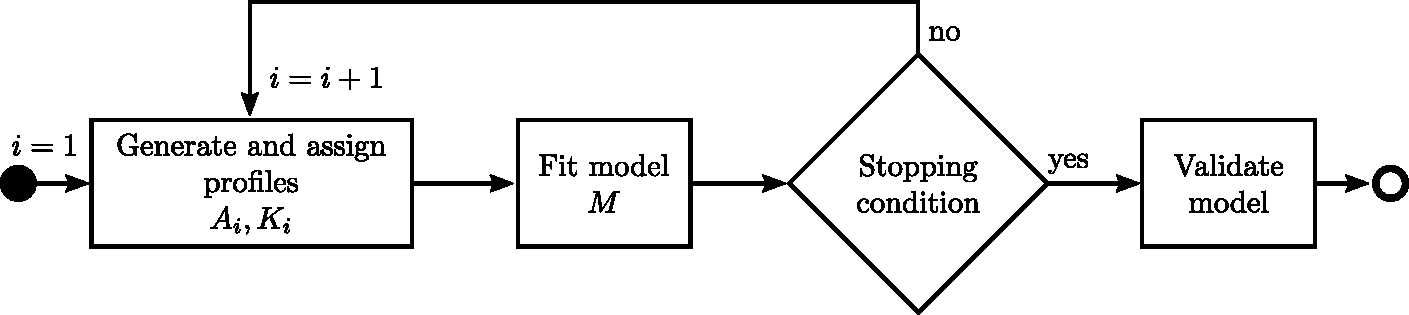
\includegraphics[scale = 0.7]{fig/expdesign1}
\caption{Protocol for inferring the parameters of an MR-Sort model}\label{fig:methodology1}
\end{figure}

The protocol consists of a series of iterations, denoted using the variable $i$.  It begins by randomly generating an initial set of member profiles, denoted with $A_i$, and having the DM assign them to categories, which are denoted with $K_i$. Especially in the initial iterations, conducting this step
interactively provides greater support for the results, as the
articulated perspective in the interview can be compared with the
model derived from the assignment examples:
a form of mixed methods triangulation \citep{Myers97}. 

The second step consists in fitting a model based on these assignments, followed by checking whether a stopping condition is met. 
The stopping condition might be based on subjective factors linked to the willingness of the DM to proceed further, or on factors linked to the fit and convergence of the model. 
If such a stopping condition is met, one proceeds to validating the model, otherwise a new iteration starts by generating an additional set of profiles. Starting with the second iteration, these profiles are generated based on the model $M$.

The second step of fitting a model over $A_j$ and $K_j$, $\forall j \in 1..i$, consists of several additional iterations which are illustrated in Figure~\ref{fig:methodology2}.

\begin{figure}
\centering
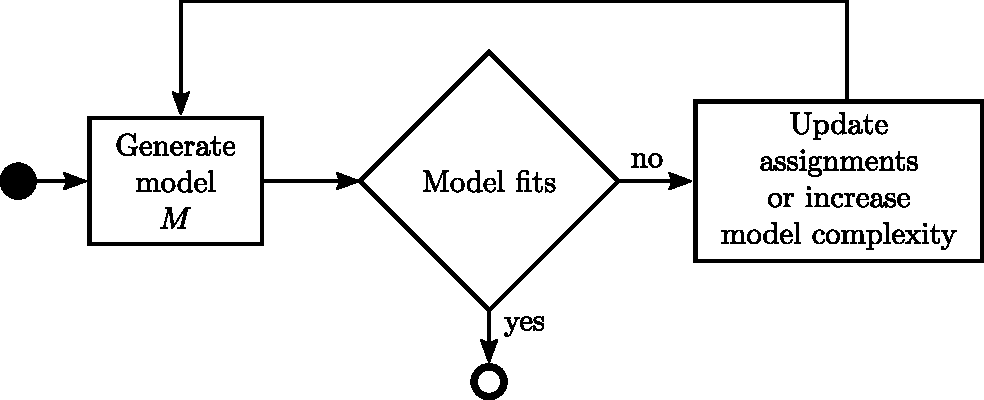
\includegraphics[scale = 0.7]{fig/expdesign2}
\caption{Protocol for fitting an MR-Sort model over a set of assignment examples}\label{fig:methodology2}
\end{figure}

Figure~\ref{fig:methodology1} begins with generating a model from all of the assignment examples from the previous iterations of the protocol. The first iteration starts with a simple MR-Sort model with no vetoes and no dictators, whereas the subsequent iterations start with the type of model previously generated. Fitting is described in Figure~\ref{fig:methodology2}. If the model fits perfectly with the assignment examples, the protocol reverts to the main sequence of steps described in Figure~\ref{fig:methodology1}. If the model does not fit, either the assignment examples are updated or the complexity of the model is increased to represent the assignments. Updating the assignment examples involves generating minimal subsets of profiles and their corresponding alternative assignments, which are then presented to the DM for validation. In increasing the complexity of the model, the {\em principle of parsimony} is applied, in that the simplest explanation is chosen, and complexity is only increased when it is necessary to fit the data. If the initial model which currently does not fit the assignments is, for example, an MR-Sort with a simple majority rule, the closest more complex model would be MR-Sort models with vetoes or dictators, followed by variants weakened by a dictator or a veto, and finally MR-Sort models with both vetoes and dictators. In cases where two equally complex models equally describe most of the assignment examples, one is chosen randomly. Once a fit is obtained, a new iteration of the initial protocol is started.

The next section illustrates with an example the three different stages of the methodology, demonstrating concretely how they can be implemented, and showing what kind of results this method produces.


\section{Experimental illustration: FLOSS}\label{sec:results}
In this section, we present a specific example of the method described in Section~\ref{sec:methodology}, namely of the FLOSS domain.

\subsection{Defining the dimensions for evaluating team members}

Universal psycho-social components were already identified in 
Section~\ref{sec:related}. Our objective was therefore to identify
technical skills specific to the domain.

The literature on skills required for FLOSS development is sparse.

\citet{david:2007:free} considered which skills software developers improve through participation in FLOSS. The study was conducted as a survey of FLOSS developers, human resource managers, and universities, in eight countries. Participants were asked to identify, from a list of 30 skills, those which developers most successfully acquired
through FLOSS participation. The skills are grouped as general, legal, managerial, and technical, but the source of the skills is not specified.
The technical category contains:
  to re-use code written by others,
  to run and maintain complex software systems,
  basic/introductory programming skills,
  to look for and fix bugs,
  to become familiar with different programming languages,
  to write code in a way that can be re-used,
  to design modular code,
  to document code, and
  to create new algorithms.

\cite{Kimmelmann13} used grounded theory on guided interviews with 
developers who participate in FLOSS development as a component of their
employment. Their team managers and human resource managers were also
interviewed. She identified three types of skills---technical,
social and personal---which were grouped according to how they
pertained to distinctive elements of FLOSS development. The technical
skills listed are:
programming, ``architectural competency,'' ``implementation of new features without disturbing others,'' quick induction into new projects, implementation of feedback, dealing with technical problems, identification of possible successful projects, gaining recognition and earning reputation, high number of quality patches, and documentation of work. 
These concepts have different levels of granularity. For instance
the concept of programming might be considered to contain the aspect
of quality patches, while the concepts of quality and quantity of patches are combined in one skill.

\cite{barcomb:2015:developers} conducted a survey to determine if
FLOSS developers had a greater preference for informal learning
styles than other software developers. They created a list of 17
highly trainable skills based on \cite{Kimmelmann13} and
\cite{david:2007:free}, which contained the following technical skills:
to evaluate the work of others;
to work on own software module alone;
to communicate with many different target groups;
to understand English, especially technical discussion;
to document code;
to clearly articulate an argument;
to understand different software architectures;
to follow discussions on mailing lists;
%% to communicate without offending others;
to write code in a way that can be reused;
basic/introductory programing skills;
to acquaint yourself with code from others;
to maintain contact with a community;
to coordinate own work with the work of others; and
%% to change criticized behavior
to understand and work with people from different cultures.

None of the lists of FLOSS skills we identified in the literature was suitable for our purpose for two reasons. First, they
are not at the same level of granularity as the psychological factors, which we
incorporated because they are universal and well-established by research, and therefore 
can be applied to any teaming situation. Second, the lists are too lengthy to allow participants to keep all attributes in mind. Considering other domains risked diluting the specific situation
we wished to observe. Therefore, we synthesized the aforementioned literature to nine
dimensions summarizing the technical skills:
% In their work describing the management of outsourced global software development in India, \citet{deshpande:2009:management} include a list of criteria which includes the skills domain knowledge, cultural background, knowledge of English, professional skills, technical experience, and other language skills, and the additional factors technical requirements and gender. These categories were derived from interviews and are clearly specific to the context.
{\em produces code of quality};
{\em understands the architecture of the code (modular code, code dependencies)};
{\em proposes implementation of new features without disturbing others};
{\em contributes a lot of commits};
{\em documents the work produced};
{\em writes clearly, in good English};
{\em implements the feedback received};
{\em is good at describing bugs}; and
{\em is good at specifying features}.
Because the next stage of the process involved validating the criteria through
interviews with DMs, the risk of overlooking a critical factor was extremely low.
At this stage there were five psychological and nine technical candidate criteria.

Next, we interviewed experts, in this case six DMs, using a semi-structured
interview and a questionnaire containing the criteria we previously 
identified. The questionnaire consisted of the information presented in
Table~\ref{tab:description-dimensions} and the question
``To which extent are these dimensions useful and important for you 
to assess the quality of a member of your community?'' for which the options were
`Very important,' `Important,' `Neutral,' `Not very important,' and
`Not important at all.' The interview script can be found in the Appendix.
%% ref{app:interview}

According to these DMs, psychological qualities were at least as important as technical capabilities. Also, the dimensions we presented were consistent and complete enough to allow for the evaluation of team members. As an additional confirmation, we reviewed the free-form answers in the interviews and compared the concepts to our list, and subsequently revised the categories to use the language of our participants. 
For example, ``commitment'' became ``commitment to the project'' based on interview data such as:
\begin{quote}
{\em
I think the level of interest in somebody is one of the biggest predictors---I 
mean if they're excited about what's going on, if they're excited about the 
mission and excited about the community that to me---that comes well before level of knowledge in the project itself or technical skill, or other things. I think that comes. If somebody's not motivated, and excited, I think the other things don't matter as much. So I would say at a simple level, just level of interest 
and excitement.} (\DB)
\end{quote}

After interviewing all six DMs, we found that no new attributes were
mentioned, suggesting that our list was sufficiently comprehensive. 
Four of the technical criteria were considered unimportant by all 
participants. We therefore decided to drop these dimensions because
they did not assist our DMs in assessing team members.
The final dimensions, five psycho-social and five technical, are presented as an illustration of the method in Table~\ref{tab:description-dimensions}. These dimensions are the same for every DM.

%% We will scale this table to the page width using adjustbox. However, we want
%% columns to wrap instead of just shrinking, so we will give each column a portion
%% of the page width which together adds up to somewhat, but not much, over the
%% actual page width. This creates the need to enforce column space with @{}.
%% Because I don't want to abuse \midrule (a big no-no with booktabs), I increased
%% arraystretch to keep the wrapped rows from bleeding into one another.

\begin{table}
\renewcommand{\arraystretch}{1.5}
\raggedright %% Ensure column wrapping doesn't give ugly spaces
\caption{Detail of the ten dimensions used to evaluate the team members}
\centering
%\begin{adjustbox}{width=1\textwidth}
\label{tab:description-dimensions}
\rotatebox{90}{
\begin{tabular}{p{.3\columnwidth}@{\hskip 6\tabcolsep}p{.4\columnwidth}@{\hskip 6\tabcolsep}p{.4\columnwidth}}
\toprule
{\bf Variable} & \multicolumn{2}{c}{\bf Description}\\
\cmidrule{2-3}
& {\it Negative} & {\it Positive}\\
\midrule

Communication skills (signal over noise ratio) & Too much noise / not enough information & Is good at providing the right level of information  \\
Commitment to the project & Unmotivated/passive in seeking answers & Is motivated and does a thorough job \\
Working with others & Tends to find fault with others & Is generally trusting, patient with people \\
Pressure and stress related managing capacity & Gets nervous and stressed easily (for instance when things do not go as expected, or when there are delays or due deliverables) & Is relaxed, handles stress, technical limitations, setbacks well \\
Creativity & Not very creative in terms of solution & Has an active imagination, proposes creative ideas/solutions \\
Quantity of code contributed & Produces few lines of code & Produces an impressive quantity of code  \\
Quality of code contributed & Tends to provide incomplete or inferior solutions & Produces efficient and well written code, without disturbing other
part of the code  \\
Global picture: understands the tools/technology/domain, and processes behind the project  & Low, does not understand beyond the talks/the modules addressed  & Understands the technical \& Non-technical fundamentals of the project  \\
Documentation \& testing & Does not document or test the code produced, or does so in a way not understandable
by others & Documents/test well and clearly the code produced \\
Contribution on other aspects than code (new features, bug description) & Does not contribute beyond code production & Very active in proposing new features, tracking and documenting bugs,
etc. \\
\bottomrule
\end{tabular}
}
%\end{adjustbox}
\renewcommand{\arraystretch}{1}
\end{table}


\subsection{Selecting the criteria for the MCDA analysis}\label{sec:results:sub:subset}

While all DMs agreed that the ten dimensions captured all attributes they would use to evaluate team members, they did not agree on the number of or the selection of criteria, as seen by their responses to the questionnaire where they
rated the relevance of the dimensions on a 5-item scale.
The exact choices of the DMs is discussed in more detail in Section~\ref{sec:discussion} and described in Table~\ref{tab:criteria}. This result advocates for a manager-based methodology, where each DM is able to identify a tailored subset of key factors from a longer list of attributes relevant to the domain.

We proceeded with each DM using the criteria they considered important or
very important. As each DM selected at least half of the criteria as
relevant, it would not have been possible for the unselected factors to
collectively deliver more relevance than the chosen factors. Limiting the
factors also improved the DM's ability to effectively consider example
team members.

\subsection{Inferring the manger's preferences}\label{sec:results:sub:model}

Although six DMs participated in our research, we have chosen to provide
a detailed account of two participants. Our reasoning was based on the goal of the paper, which is to present the methodology and demonstrate how it can provide new results for the DM and for researchers on the interaction between a DM and virtual team members. We considered it more important to describe in detail a minimal set of examples, rather than to discuss all cases superficially or to significantly lengthen the paper without providing new information about the process, potentially creating the false impression that we are conducting a qualitative study of FLOSS DMs. The extension of the number of DM beyond the two we present and the six total interviews toward more general studies is of course the next step, which will be described further in Section~\ref{sec:discussion}.

 We chose to report on \GJ and \DB for two reasons.
First, these DMs selected the same criteria in the previous phase,
which allows us to illustrate how the method performs when the DMs
are concerned with the same dimensions. Differences between the two
inferred preference models demonstrates the difficulty of creating a
general evaluation, and the benefit in a customized approach. Second,
\GJ and \DB both selected fewer dimensions than other participants.
With fewer dimensions, the models are simpler and the differences between
the models are more readily evident.
The five dimensions chosen by \GJ and \DB were:
\begin{itemize}
\item Commitment to the project ($c_1$), psycho-sociological;
\item Ability to work with others ($c_2$), psycho-sociological;
\item Quality of produced code ($c_3$), technical;
\item Understanding of the tools, technologies, domain and process behind the project ($c_4$), technical;
\item Documentation skills ($c_5$), technical.
\end{itemize}

Mock profiles---alternatives in an MCDA context---were created using the aforementioned five dimensions, with each trait described using a five-level ordinal scale ranging from very bad to very good ($\{vb, b, n, g, vg\}$). The DMs rated these profiles as good, neutral and bad (hence \\$K = \{Bad, Neutral, Good\}$).

\subsubsection{Inferring the preference model of \GJ}

We started the first iteration by generating an initial set of 25 team member profiles, which \GJ assigned to one of the categories in $K$, while explaining his reasoning to one of the paper's authors. \GJ's assignments are illustrated in Table~\ref{tab:ex1-data1}.

\begin{table}
\caption{The initial set of contributor profiles and their assignment by \GJ;}\label{tab:ex1-data1}
\setlength{\tabcolsep}{4pt}
\tabulinesep=2pt
\begin{minipage}[t]{.49\textwidth}
\vspace{0pt}

\centering

\begin{tabu}{c|ccccc|c}
Profile& \multicolumn{5}{c|}{Criteria} & Assigned\\
number& $c_1$ & $c_2$ & $c_3$ & $c_4$ & $c_5$ & category \\\hline
1 &vg & g &vb &vg & n & Bad\\
2 & b &vg & n &vb & n & Neutral\\
3 & b & b & b & b & g & Bad\\
4 & b & b &vb &vg & n & Bad\\
5 & g &vb &vg & b & b & Neutral\\
6 &vg & g &vg & n &vg & Good\\
7 & g & n & b & n &vg & Neutral\\
8 & n & n & g & b & g & Good\\
9 & n &vg & n & g & b & Bad\\
10&vb & g &vg &vb & b & Bad\\
11& g & g & g &vb &vg & Good\\
12& n & g & g &vb & g & Neutral\\
13& g & g & n & n &vb & Bad
\end{tabu}
\end{minipage}
\hfill
\begin{minipage}[t]{.49\textwidth}
\vspace{0pt}

\centering

\begin{tabu}{c|ccccc|c}
Profile& \multicolumn{5}{c|}{Criteria} & Assigned\\
number& $c_1$ & $c_2$ & $c_3$ & $c_4$ & $c_5$ & category \\\hline
14&vg & n &vb & b & g & Bad\\
15& n & b & b &vb & n & Bad\\
16& b &vg & g &vg &vb & Bad\\
17& n & b & n & g & n & Bad\\
18&vg &vb &vg & g & b & Neutral\\
19&vg &vb & n & n &vb & Bad\\
20&vb &vg &vg & b &vg & Neutral\\
21&vb & n &vb & n &vb & Bad\\
22&vb & b &vb &vg & g & Bad\\
23&vb &vb & g & g &vg & Neutral\\
24& g &vb & b & g &vb & Bad\\
25& b & n & b &vg & b & Bad
\end{tabu}
\end{minipage}
\end{table}

We then tried to fit these assignment examples with an MR-Sort model with a simple majority rule, but only 23 of the 25 responses could be fit. We therefore proceeded to generate a series of sets of the two profiles along with their alternative class assignments which would allow this model to fit. These sets are illustrated in Table~\ref{tab:ex1-altassig1}.

\begin{table}
\caption{The alternative assignments for an MR-Sort model within the first iteration of the inference protocol for \GJ.}\label{tab:ex1-altassig1}
\setlength{\tabcolsep}{4pt}
\tabulinesep=2pt

\centering

\begin{tabu}{cc|ccccc|cc}
&Profile& \multicolumn{5}{c}{Criteria} & \multicolumn{2}{c}{Category} \\
%&number& $c_1$ & $c_2$ & $c_3$ & $c_4$ & $c_5$ & \multicolumn{1}{c}{CM} & \multicolumn{1}{c}{MR-Sort} \\\hline
&number& $c_1$ & $c_2$ & $c_3$ & $c_4$ & $c_5$ & \multicolumn{1}{c}{original} & \multicolumn{1}{c}{alternative} \\\hline
\multirow{2}{*}{First set}& 2 &  b & vg & n & vb & n &  Neutral & Bad \\
& 8 & n & n & g & b & g & Good & Neutral \\[2pt]
\multirow{2}{*}{Second set}& 2 & b & vg & n & vb & n &  Neutral & Bad \\
& 11 & g & g & g & vb & vg & Good & Neutral \\[2pt]
\multirow{2}{*}{Third set}& 2 & b & vg & n & vb & n &  Neutral & Bad \\
& 12 & n & vg & g & vb & g & Neutral & Good
\end{tabu}
% \begin{tabular}{ccccccc||c|c}
% &Profile& \multicolumn{5}{c}{Criteria} & \multicolumn{2}{c}{Category} \\
% &number& $c_1$ & $c_2$ & $c_3$ & $c_4$ & $c_5$ & \multicolumn{1}{c}{original} & \multicolumn{1}{c}{alternative} \\\hline
% \multirow{2}{*}{First set}&         2 &        bad &     v.good &    neutral &      v.bad &    neutral &  Neutral & Bad \\
% &         8 &    neutral &    neutral &       good &        bad &       good & Good & Neutral \\\hline
         
% \multirow{2}{*}{Second set}&         2 &        bad &     v.good &    neutral &      v.bad &    neutral &  Neutral & Bad \\
% &        11 &       good &       good &       good &      v.bad &     v.good & Good & Neutral \\\hline
        
% \multirow{2}{*}{Third set}&         2 &        bad &     v.good &    neutral &      v.bad &    neutral &  Neutral & Bad \\
% &        12 &    neutral &     v.good &       good &      v.bad &       good & Neutral & Good  \\
        
% \end{tabular}
\end{table}

Using these sets, we devised a series of questions for the DM to simplify his task of considering these alternative assignments. As the second team member profile appeared in all three sets, we asked if he would agree to change his assignment from Neutral to Bad. \GJ agreed to change his assignment, and confirmed that he had initially hesitated between these two categories. We continued by asking him if he would agree to changing the assignments of any of the other profiles from the three sets, but he disagreed. Consequently we increased the complexity of the model and found that an MR-Sort model with vetoes was able to capture all 25 profile assignments.

This ended the step of fitting a model for the first iteration, leading to the model illustrated in Figure~\ref{fig:ex1-model1}. The first diagram shows the limit between the Bad and Neutral classes, while the second shows the boundary between Neutral and Good. The lines correspond to the limits, while the dark regions represent the range of values which would trigger a veto. At this point, the model is not yet presented to the DM so no attempt is made to derive examples from it.

\begin{figure}
\centering

\begin{minipage}[c]{0.4\columnwidth}
\vspace{0pt}
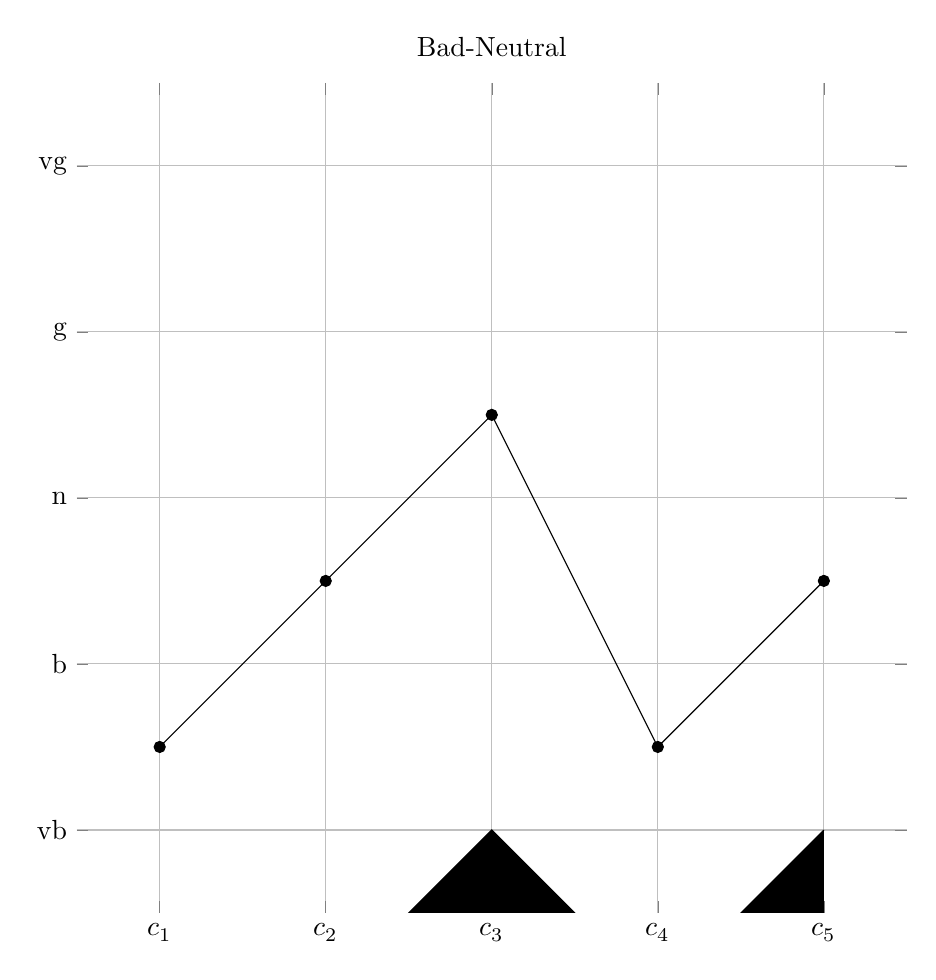
\begin{tikzpicture}
\begin{axis}[title ={Bad-Neutral}, height=\textwidth,width=\textwidth, xmin = 0.5, xmax = 5.5, ymin = -2.5, ymax = 2.5, every axis x label/.style={at={(ticklabel* cs:0.97)},anchor=south},xtick={1,2,3,4,5}, xticklabels={$c_1$,$c_2$,$c_3$,$c_4$,$c_5$}, ytick={-2,-1,0,1,2}, xmajorgrids = true, axis line style = { draw = none }, yticklabels = {vb, b, n, g, vg}, ymajorgrids = true]
\addplot[name path=T]
coordinates {
	(1,3)
	(2,3)
	(3,3)
	(4,3)
	(5,3)
};
\addplot[name path=B]
coordinates {
	(1,-3)
	(2,-3)
	(3,-3)
	(4,-3)
	(5,-3)
};
\addplot[name path=P, black, solid, mark = *]
coordinates {
	(1,-1.5)
	(2,-0.5)
	(3,0.5)
	(4,-1.5)
	(5,-0.5)
};
\addplot[name path=V]
coordinates {
	(0,-3)
	(1,-3)
	(2,-3)
	(3,-2)
	(4,-3)
	(5,-2)
};
\addplot[black] fill between[of=V and B];
\end{axis}
\end{tikzpicture}
\end{minipage}
\begin{minipage}[c]{0.4\columnwidth}
\vspace{0pt}

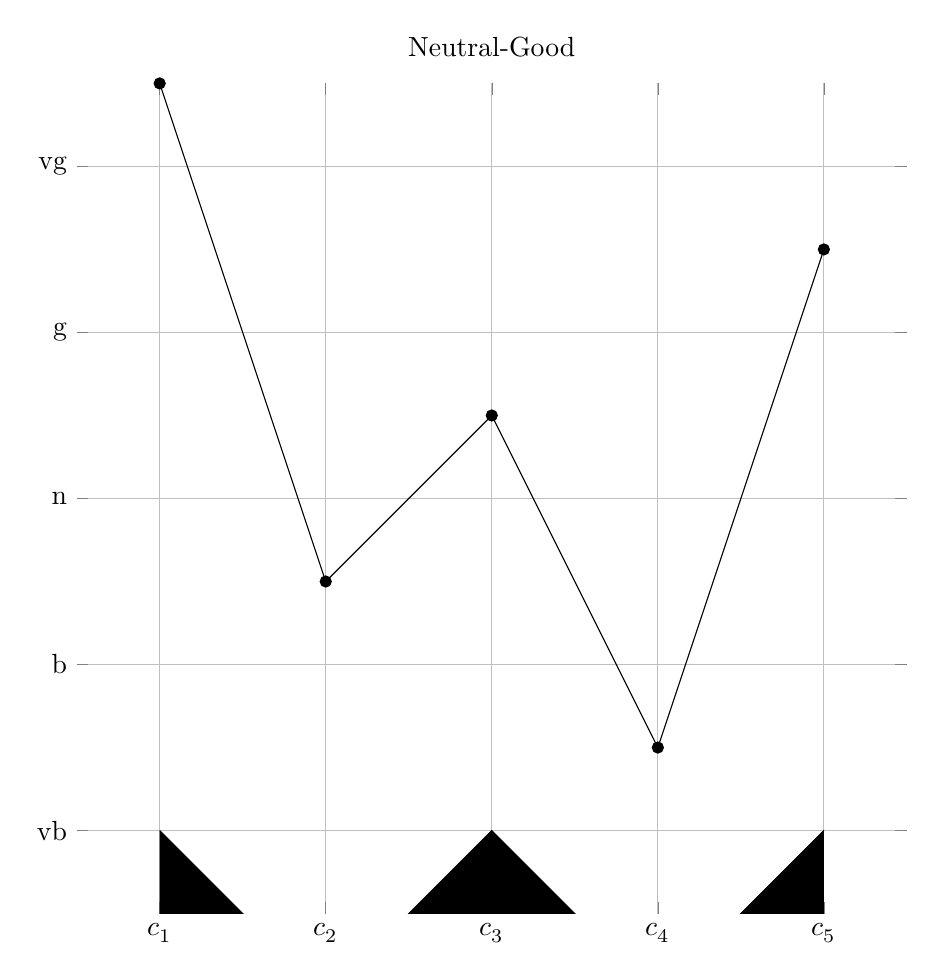
\begin{tikzpicture}
\begin{axis}[title ={Neutral-Good}, height=\textwidth,width=\textwidth, xmin = 0.5, xmax = 5.5, ymin = -2.5, ymax = 2.5, every axis x label/.style={at={(ticklabel* cs:0.97)},anchor=south},xtick={1,2,3,4,5}, xticklabels={$c_1$,$c_2$,$c_3$,$c_4$,$c_5$}, ytick={-2,-1,0,1,2}, xmajorgrids = true, axis line style = { draw = none }, yticklabels = {vb, b, n, g, vg}, ymajorgrids = true]
\addplot[name path=T]
coordinates {
	(1,3)
	(2,3)
	(3,3)
	(4,3)
	(5,3)
};
\addplot[name path=B]
coordinates {
	(1,-3)
	(2,-3)
	(3,-3)
	(4,-3)
	(5,-3)
};
\addplot[name path=P, black, solid, mark = *]
coordinates {
	(1,2.5)
	(2,-0.5)
	(3,0.5)
	(4,-1.5)
	(5,1.5)
};
\addplot[name path=V]
coordinates {
	(1,-2)
	(2,-3)
	(3,-2)
	(4,-3)
	(5,-2)
};
\addplot[black] fill between[of=V and B];
\end{axis}
\end{tikzpicture}
\end{minipage}
\begin{minipage}[c]{0.07\columnwidth}
\vspace{0pt}

\begin{tabular}{c|c}
$\lambda$ & 0.6 \\\hline
$c_1$ & 0.20 \\
$c_2$ & 0.20 \\
$c_3$ & 0.25 \\
$c_4$ & 0.15 \\
$c_5$ & 0.20 \\
\end{tabular}
\end{minipage}

\caption{First preference model of \GJ (MR-Sort with vetoes).}\label{fig:ex1-model1}
\end{figure}

We were therefore able to complete the first iteration of our protocol and proceeded to check if a stopping condition was met. The assignment examples did not restrict the model very much, and, as \GJ was willing to continue, we began a second iteration.

An additional set of 10 profiles were generated, based on the previously created model. This set was presented to \GJ who assigned them as seen in Table~\ref{tab:ex1-data2}. This was again done interactively with a researcher present.

\begin{table}
\caption{The second set of contributor profiles and their assignment by \GJ.}\label{tab:ex1-data2}
\setlength{\tabcolsep}{4pt}
\tabulinesep=2pt
\begin{minipage}[t]{.49\textwidth}
\vspace{0pt}

\centering

\begin{tabu}{c|ccccc|c}
Profile& \multicolumn{5}{c|}{Criteria} & Assigned\\
number& $c_1$ & $c_2$ & $c_3$ & $c_4$ & $c_5$ & category \\\hline
26 &vg & g &n &b & b & Bad\\
27 &vg & b & n &vg & b & Bad\\
28 &vg & b & n & b & vg & Neutral\\
29 &vb &vg & n & vg & b & Bad\\
30 &vb &vg & n & b & vg & Bad
\end{tabu}
\end{minipage}
\hfill
\begin{minipage}[t]{.49\textwidth}
\vspace{0pt}

\centering

\begin{tabu}{c|ccccc|c}
Profile& \multicolumn{5}{c|}{Criteria} & Assigned\\
number& $c_1$ & $c_2$ & $c_3$ & $c_4$ & $c_5$ & category \\\hline
31&vb & b &vg &vg & b & Bad\\
32&vb & b & n &vg & vg & Bad\\
33&vg &vg &vb &vg &vg & Neutral\\
34&vg &vg &vg &vg &vb & Good\\
35&b &vb & g &vb & n & Neutral
\end{tabu}
\end{minipage}

% \begin{tabular}{cccccc||c}
% Profile& \multicolumn{5}{c}{Criteria} & \multicolumn{1}{c}{Category assignment}\\
% number& $c_1$ & $c_2$ & $c_3$ & $c_4$ & $c_5$ & \multicolumn{1}{c}{\GJ} \\\hline
% 26& v.good & v.good & neutral & bad & bad & Bad \\\hline
% 27& v.good & bad & neutral & v.good & bad & Bad \\\hline
% 28& v.good & bad & neutral & bad & v.good & Neutral \\\hline
% 29& v.bad & v.good & neutral & v.good & bad & Bad \\\hline
% 30& v.bad & v.good & neutral & bad & v.good & Bad \\\hline
% 31& v.bad & bad & v.good & v.good & bad & Bad \\\hline
% 32& v.bad & bad & neutral & v.good & v.good & Bad \\\hline
% 33& v.good & v.good & v.bad & v.good & v.good & Neutral \\\hline
% 34& v.good & v.good & v.good & v.good & v.bad & Good \\\hline
% 35& bad & v.bad & good & v.bad & neutral & Neutral \\\hline
% \end{tabular}
\end{table}

We combined the initial set of 25 profiles with the new set of 10 and tested whether an MR-Sort model with vetoes was still able to capture them. This model did not completely fit the assignments. We therefore proceeded to check if \GJ had any hesitations in his assignments which would allow this model to be used. Five sets of alternative class assignments, shown in Table~\ref{tab:ex1-altassig2}, were generated to explore this possibility.

\begin{table}
\caption{The alternative assignments for an MR-Sort model with vetoes within the second iteration of the inference protocol for \GJ.}\label{tab:ex1-altassig2}
\setlength{\tabcolsep}{4pt}
\tabulinesep=2pt

\centering

\begin{tabu}{cc|ccccc|cc}
&Profile& \multicolumn{5}{c}{Criteria} & \multicolumn{2}{|c}{Category} \\
&number& $c_1$ & $c_2$ & $c_3$ & $c_4$ & $c_5$ & \multicolumn{1}{c}{original} & \multicolumn{1}{c}{alternative} \\\hline
\multirow{2}{*}{First set}&         2 &        b &     vg &    n &      vb &    n &  Neutral & Bad \\
&        16 &        b &     vg &       g &     vg &      vb  &  Bad & Neutral \\[2pt]
\multirow{2}{*}{Second set}&         2 &        b &     vg &    n &      vb &    n  &  Neutral & Bad \\
&        33 &     vg &     vg &      vb &     vg &     vg  &  Neutral & Bad \\[2pt]
\multirow{2}{*}{Third set}&         2 &        b &     vg &    n &      vb &    n  &  Neutral & Bad \\
&        34 &     vg &     vg &     vg &     vg &      vb  &  Good & Bad \\[2pt]
\multirow{2}{*}{Fourth set}&         2 &        b &     vg &    n &      vb &    n  &  Neutral & Bad \\
&                 35 &        b &      vb &       g &      vb  & n  &  Neutral & Bad \\[2pt]
\multirow{2}{*}{Fifth set}&        30 &      vb &     vg &    n &        b &     vg  &  Bad & Neutral \\
&        33 &     vg &     vg &      vb &     vg &     vg  &  Neutral & Bad
\end{tabu}
% \begin{tabular}{ccccccc|cc}
% &Profile& \multicolumn{5}{c}{Criteria} & \multicolumn{2}{|c}{Category} \\
% &number& $c_1$ & $c_2$ & $c_3$ & $c_4$ & $c_5$ & \multicolumn{1}{c}{original} & \multicolumn{1}{c}{alternative} \\\hline
% \multirow{2}{*}{First set}&         2 &        bad &     v.good &    neutral &      v.bad &    neutral &  Neutral & Bad \\
% &        16 &        bad &     v.good &       good &     v.good &      v.bad  &  Bad & Neutral \\\hline
        
% \multirow{2}{*}{Second set}&         2 &        bad &     v.good &    neutral &      v.bad &    neutral  &  Neutral & Bad \\
% &        33 &     v.good &     v.good &      v.bad &     v.good &     v.good  &  Neutral & Bad \\\hline
         
% \multirow{2}{*}{Third set}&         2 &        bad &     v.good &    neutral &      v.bad &    neutral  &  Neutral & Bad \\
% &        34 &     v.good &     v.good &     v.good &     v.good &      v.bad  &  Good & Bad \\\hline
         
% \multirow{2}{*}{Fourth set}&         2 &        bad &     v.good &    neutral &      v.bad &    neutral  &  Neutral & Bad \\
% &                 35 &        bad &      v.bad &       good &      v.bad  & neutral  &  Neutral & Bad \\\hline
                 
% \multirow{2}{*}{Fifth set}&        30 &      v.bad &     v.good &    neutral &        bad &     v.good  &  Bad & Neutral \\
% &        33 &     v.good &     v.good &      v.bad &     v.good &     v.good  &  Neutral & Bad \\\hline
% \end{tabular}
\end{table}

We observed that the first four sets contained the second team member profile, which \GJ had already agreed to change. Therefore, we continued by first asking if he would also agree to an alternative assignment for one of the remaining profiles in these sets. \GJ did not accept changing the assignment profiles 16, 33 or 34, especially for the third set where the alternative assignment strongly contradicted the initial assignment. However, \GJ agreed to change the assignment of profile 35, so we continued to use an MR-Sort model with vetoes, as depicted in Figure~\ref{fig:ex1-model2}.

\begin{figure}
\centering

\begin{minipage}[c]{0.4\columnwidth}
\vspace{0pt}

\begin{tikzpicture}
\begin{axis}[title ={Bad-Neutral}, height=\textwidth,width=\textwidth, xmin = 0.5, xmax = 5.5, ymin = -2.5, ymax = 2.5, every axis x label/.style={at={(ticklabel* cs:0.97)},anchor=south},xtick={1,2,3,4,5}, xticklabels={$c_1$,$c_2$,$c_3$,$c_4$,$c_5$}, ytick={-2,-1,0,1,2}, xmajorgrids = true, axis line style = { draw = none }, yticklabels = {vb, b, n, g, vg}, ymajorgrids = true]
\addplot[name path=T]
coordinates {
	(1,3)
	(2,3)
	(3,3)
	(4,3)
	(5,3)
};
\addplot[name path=B]
coordinates {
	(1,-3)
	(2,-3)
	(3,-3)
	(4,-3)
	(5,-3)
};
\addplot[name path=P, black, solid, mark = *]
coordinates {
	(1,-0.5)
	(2,-2)
	(3,0.5)
	(4,-1.5)
	(5,1.5)
};
\addplot[name path=V]
coordinates {
	(0,-3)
	(1,-3)
	(2,-3)
	(3,-3)
	(4,-3)
	(5,-3)
};
\addplot[black] fill between[of=V and B];
\end{axis}
\end{tikzpicture}
\end{minipage}
\begin{minipage}[c]{0.4\columnwidth}
\vspace{0pt}

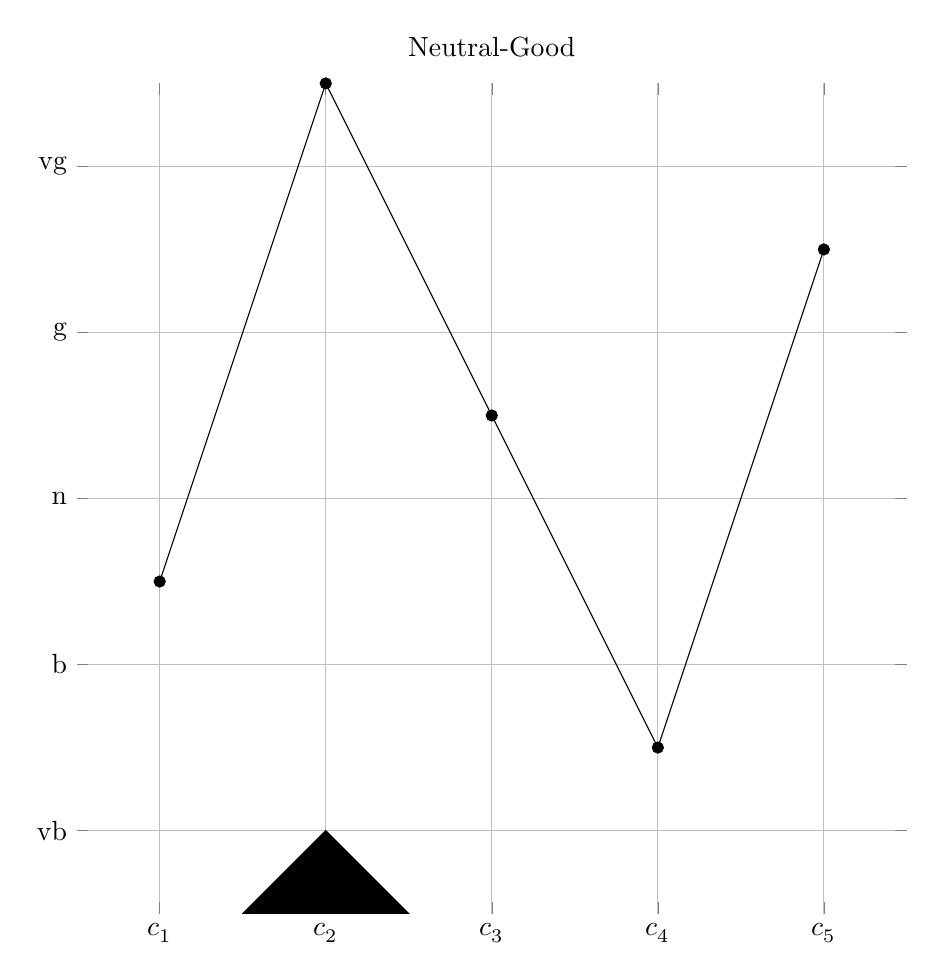
\begin{tikzpicture}
\begin{axis}[title ={Neutral-Good}, height=\textwidth,width=\textwidth, xmin = 0.5, xmax = 5.5, ymin = -2.5, ymax = 2.5, every axis x label/.style={at={(ticklabel* cs:0.97)},anchor=south},xtick={1,2,3,4,5}, xticklabels={$c_1$,$c_2$,$c_3$,$c_4$,$c_5$}, ytick={-2,-1,0,1,2}, xmajorgrids = true, axis line style = { draw = none }, yticklabels = {vb, b, n, g, vg}, ymajorgrids = true]
\addplot[name path=T]
coordinates {
	(1,3)
	(2,3)
	(3,3)
	(4,3)
	(5,3)
};
\addplot[name path=B]
coordinates {
	(1,-3)
	(2,-3)
	(3,-3)
	(4,-3)
	(5,-3)
};
\addplot[name path=P, black, solid, mark = *]
coordinates {
	(1,-0.5)
	(2,2.5)
	(3,0.5)
	(4,-1.5)
	(5,1.5)
};
\addplot[name path=V]
coordinates {
	(1,-3)
	(2,-2)
	(3,-3)
	(4,-3)
	(5,-3)
};
\addplot[black] fill between[of=V and B];
\end{axis}
\end{tikzpicture}
\end{minipage}
\begin{minipage}[c]{0.07\columnwidth}
\vspace{0pt}

\begin{tabular}{c|c}
$\lambda$ & 0.6 \\\hline
$c_1$ & 0.25 \\
$c_2$ & 0.13 \\
$c_3$ & 0.25 \\
$c_4$ & 0.13 \\
$c_5$ & 0.13 \\
\end{tabular}
\end{minipage}
% \begin{tikzpicture}
% \begin{axis}[title ={Bad-Neutral}, height=0.42\columnwidth,width=.42\columnwidth, xmin = 0.5, xmax = 5.5, ymin = -2.5, ymax = 2.5, every axis x label/.style={at={(ticklabel* cs:0.97)},anchor=south},xtick={1,2,3,4,5}, xticklabels={$c_1$,$c_2$,$c_3$,$c_4$,$c_5$}, ytick={-2,-1,0,1,2}, xmajorgrids = true, axis line style = { draw = none }, yticklabels = {vb, b, n, g, vg}, ymajorgrids = true]
% \addplot[name path=T]
% coordinates {
% 	(1,3)
% 	(2,3)
% 	(3,3)
% 	(4,3)
% 	(5,3)
% };
% \addplot[name path=B]
% coordinates {
% 	(1,-3)
% 	(2,-3)
% 	(3,-3)
% 	(4,-3)
% 	(5,-3)
% };
% \addplot[name path=P, black, solid, mark = *]
% coordinates {
% 	(1,-0.5)
% 	(2,-2)
% 	(3,0.5)
% 	(4,-1.5)
% 	(5,1.5)
% };
% \addplot[name path=V]
% coordinates {
% 	(0,-3)
% 	(1,-3)
% 	(2,-3)
% 	(3,-3)
% 	(4,-3)
% 	(5,-3)
% };
% \addplot[black] fill between[of=V and B];
% \end{axis}
% \end{tikzpicture}
% \begin{tikzpicture}
% \begin{axis}[title ={Neutral-Good}, height=0.42\columnwidth,width=.42\columnwidth, xmin = 0.5, xmax = 5.5, ymin = -2.5, ymax = 2.5, every axis x label/.style={at={(ticklabel* cs:0.97)},anchor=south},xtick={1,2,3,4,5}, xticklabels={$c_1$,$c_2$,$c_3$,$c_4$,$c_5$}, ytick={-2,-1,0,1,2}, xmajorgrids = true, axis line style = { draw = none }, yticklabels = {vb, b, n, g, vg}, ymajorgrids = true]
% \addplot[name path=T]
% coordinates {
% 	(1,3)
% 	(2,3)
% 	(3,3)
% 	(4,3)
% 	(5,3)
% };
% \addplot[name path=B]
% coordinates {
% 	(1,-3)
% 	(2,-3)
% 	(3,-3)
% 	(4,-3)
% 	(5,-3)
% };
% \addplot[name path=P, black, solid, mark = *]
% coordinates {
% 	(1,-0.5)
% 	(2,2.5)
% 	(3,0.5)
% 	(4,-1.5)
% 	(5,1.5)
% };
% \addplot[name path=V]
% coordinates {
% 	(1,-3)
% 	(2,-2)
% 	(3,-3)
% 	(4,-3)
% 	(5,-3)
% };
% \addplot[black] fill between[of=V and B];
% \end{axis}
% \end{tikzpicture}

% {\scriptsize
	
% \begin{tabular}{cccccc}
% $\lambda$ & $c_1$ & $c_2$& $c_3$ & $c_4$ & $c_5$\\
% \hline
% $0.6$ & $0.25$ & $0.13$ & $0.25$ & $0.13$ & $0.13$
% \end{tabular}
% }
\caption{Second preference model of \GJ (MR-Sort with vetoes).}\label{fig:ex1-model2}
\end{figure}

With the second iteration of preference modeling completed, we checked to determine if the process was complete. Given the existing model, a bare 8 profiles would suffice to express the limits. \GJ agreed to another iteration.

We generated the $8$ new profiles, and asked \GJ to assign them during an interview. The results of this assignment are presented in Table~\ref{tab:ex1-data3}.

\begin{table}
\caption{The third set of contributor profiles and their assignment by \GJ.}\label{tab:ex1-data3}
\setlength{\tabcolsep}{4pt}
\tabulinesep=2pt
\begin{minipage}[t]{.49\textwidth}
\vspace{0pt}

\centering

\begin{tabu}{c|ccccc|c}
Profile& \multicolumn{5}{c}{Criteria} &\\
number& $c_1$ & $c_2$ & $c_3$ & $c_4$ & $c_5$ & Category \\\hline
36 &b & vg &n &vg & g & Bad\\
37 &n & b & g &vb & vg & Neutral\\
38 &n & vb & vb & b & vg & Bad\\
39 &vb &vb & g & b & vg & Neutral
\end{tabu}
\end{minipage}
\hfill
\begin{minipage}[t]{.49\textwidth}
\vspace{0pt}

\centering

\begin{tabu}{c|ccccc|c}
Profile& \multicolumn{5}{c}{Criteria} &\\
number& $c_1$ & $c_2$ & $c_3$ & $c_4$ & $c_5$ & Category \\\hline
40&vg & vb &vg &vg & vg & Good\\
41&n & vb & g &vb & vb & Bad\\
42&n &b &g &b &vb & Bad\\
43&b &vg &n &vb &vg & Good
\end{tabu}
\end{minipage}
% \begin{tabular}{cccccc||c}
% Profile& \multicolumn{5}{c}{Criteria} & \multicolumn{1}{c}{Category assignment}\\
% 36 & bad & v.good & neutral & v.good & good & Bad \\\hline
% 37 & neutral & bad & good & v.bad & v.good & Neutral \\\hline
% 38 & neutral & v.bad & v.bad & bad & v.good & Bad \\\hline
% 39 & v.bad & v.bad & good & bad & v.good & Neutral \\\hline
% 40 & v.good & v.bad & v.good & v.good & v.good & Good \\\hline
% 41 & neutral & v.bad & good & v.bad & v.bad & Bad \\\hline
% 42 & neutral & bad & good & bad & v.bad & Bad \\\hline
% 43 & bad & v.good & neutral & v.bad & v.good & Bad \\\hline
% \end{tabular}
\end{table}

After adding the new profiles and their assignments to the existing ones, we found that an MR-Sort model with vetoes was not able to represent all of the assignments. We generated three possible profile changes, as shown in Table~\ref{tab:ex1-altassig3}.

\begin{table}
\caption{The alternative assignments for an MR-Sort model with vetoes within the third iteration of the inference protocol for \GJ.}\label{tab:ex1-altassig3}
\setlength{\tabcolsep}{4pt}
\tabulinesep=2pt

\centering

\begin{tabu}{cc|ccccc|cc}
&Profile& \multicolumn{5}{c}{Criteria} & \multicolumn{2}{|c}{Category} \\
&number& $c_1$ & $c_2$ & $c_3$ & $c_4$ & $c_5$ & \multicolumn{1}{c}{original} & \multicolumn{1}{c}{alternative} \\\hline
\multirow{1}{*}{First set}&         14 &     vg &    n &      vb &        b &       g &  Bad & Neutral \\[2pt]
\multirow{1}{*}{Second set}&        33 &     vg &    vg &      vb &     vg &     vg &  Neutral & Bad \\[2pt]
\multirow{1}{*}{Third set}&         34 &     vg &     vg &     vg &     vg & vb & Good & Bad
\end{tabu}
% \begin{tabular}{ccccccc|cc}
% &Profile& \multicolumn{5}{c}{Criteria} & \multicolumn{2}{|c}{Category} \\
% &number& $c_1$ & $c_2$ & $c_3$ & $c_4$ & $c_5$ & \multicolumn{1}{c}{original} & \multicolumn{1}{c}{alternative} \\\hline
% \multirow{1}{*}{First set}&         14 &     v.good &    neutral &      v.bad &        bad &       good &  Bad & Neutral \\\hline
        
% \multirow{1}{*}{Second set}&        33 &     v.good &     v.good &      v.bad &     v.good &     v.good &  Neutral & Bad \\\hline
         
% \multirow{1}{*}{Third set}&         34 &     v.good &     v.good &     v.good &     v.good & v.bad & Good & Bad \\\hline
% \end{tabular}
\end{table}

Profiles 33 and 34 reoccurred, but we were already aware that \GJ did not want to change these profiles. Therefore we only inquired on the possibility of changing profile 14. \GJ felt strongly about retaining his initial assessment, motivating us to test a more complex model. We applied an MR-Sort model with vetoes weakened by dictators, as it was closest to our previous model. This model, illustrated in Figure~\ref{fig:ex1-model3}, was able to reflect all of \GJ's assignments from the first three iterations.

\begin{figure}
\centering

\begin{minipage}[c]{0.4\columnwidth}
\vspace{0pt}

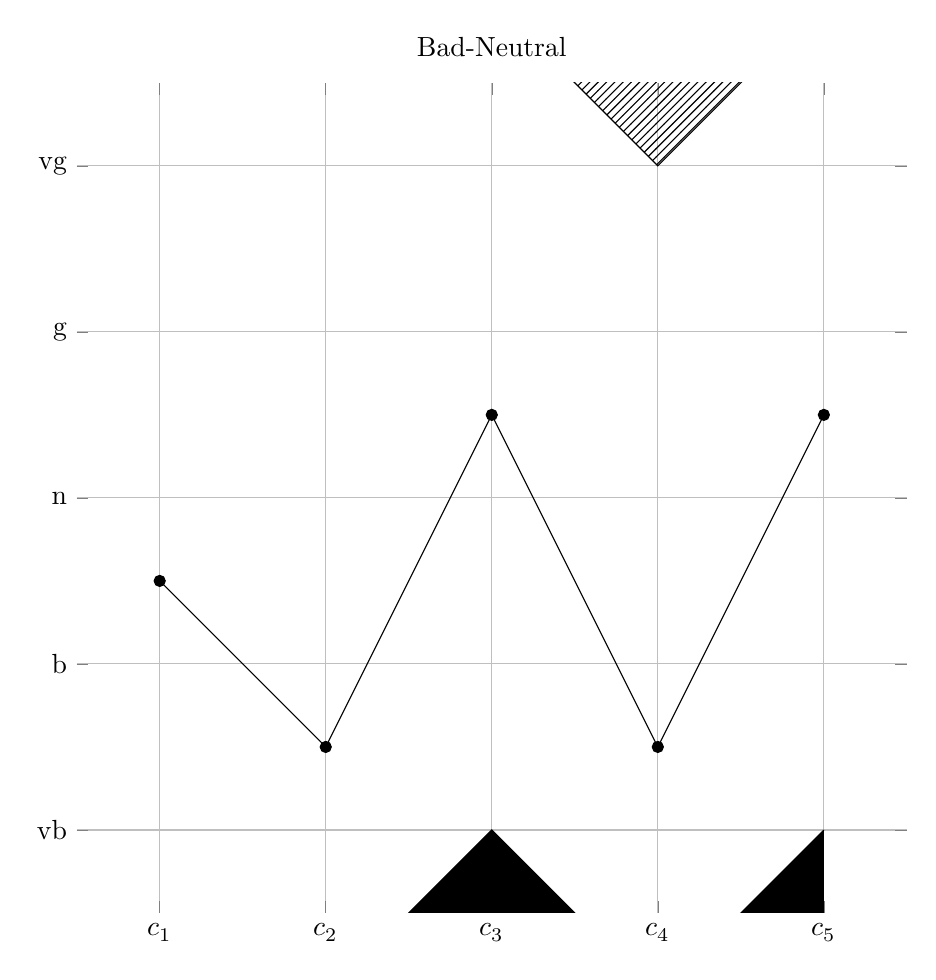
\begin{tikzpicture}
\begin{axis}[title ={Bad-Neutral}, height=\textwidth,width=\textwidth, xmin = 0.5, xmax = 5.5, ymin = -2.5, ymax = 2.5, every axis x label/.style={at={(ticklabel* cs:0.97)},anchor=south},xtick={1,2,3,4,5}, xticklabels={$c_1$,$c_2$,$c_3$,$c_4$,$c_5$}, ytick={-2,-1,0,1,2}, xmajorgrids = true, axis line style = { draw = none }, yticklabels = {vb, b, n, g, vg}, ymajorgrids = true]
\addplot[name path=T]
coordinates {
	(1,3)
	(2,3)
	(3,3)
	(4,3)
	(5,3)
};
\addplot[name path=B]
coordinates {
	(1,-3)
	(2,-3)
	(3,-3)
	(4,-3)
	(5,-3)
};
\addplot[name path=P, black, solid, mark = *]
coordinates {
	(1,-0.5)
	(2,-1.5)
	(3,0.5)
	(4,-1.5)
	(5,0.5)
};
\addplot[name path=V]
coordinates {
	(1,-3)
	(2,-3)
	(3,-2)
	(4,-3)
	(5,-2)
};
\addplot[name path=D]
coordinates {
	(1,3)
	(2,3)
	(3,3)
	(4,2)
	(5,3)
};
\addplot[black] fill between[of=V and B];
\addplot[pattern = north east lines] fill between[of=D and T];
\end{axis}
\end{tikzpicture}
\end{minipage}
\begin{minipage}[c]{0.4\columnwidth}
\vspace{0pt}

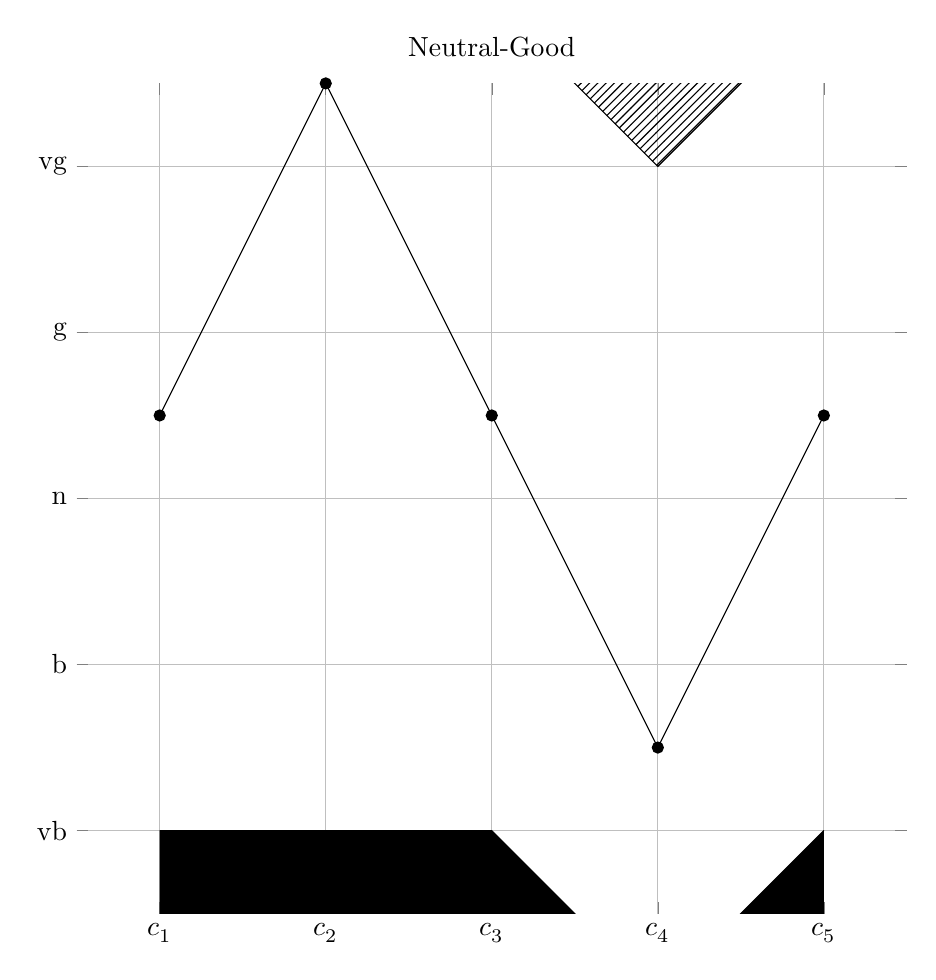
\begin{tikzpicture}
\begin{axis}[title ={Neutral-Good}, height=\textwidth,width=\textwidth, xmin = 0.5, xmax = 5.5, ymin = -2.5, ymax = 2.5, every axis x label/.style={at={(ticklabel* cs:0.97)},anchor=south},xtick={1,2,3,4,5}, xticklabels={$c_1$,$c_2$,$c_3$,$c_4$,$c_5$}, ytick={-2,-1,0,1,2}, xmajorgrids = true, axis line style = { draw = none }, yticklabels = {vb, b, n, g, vg}, ymajorgrids = true]
\addplot[name path=T]
coordinates {
	(1,3)
	(2,3)
	(3,3)
	(4,3)
	(5,3)
};
\addplot[name path=B]
coordinates {
	(1,-3)
	(2,-3)
	(3,-3)
	(4,-3)
	(5,-3)
};
\addplot[name path=P, black, solid, mark = *]
coordinates {
	(1,0.5)
	(2,2.5)
	(3,0.5)
	(4,-1.5)
	(5,0.5)
};
\addplot[name path=V]
coordinates {
	(1,-2)
	(2,-2)
	(3,-2)
	(4,-3)
	(5,-2)
};
\addplot[name path=D]
coordinates {
	(1,3)
	(2,3)
	(3,3)
	(4,2)
	(5,3)
};
\addplot[black] fill between[of=V and B];
\addplot[pattern = north east lines] fill between[of=D and T];
\end{axis}
\end{tikzpicture}
\end{minipage}
\begin{minipage}[c]{0.07\columnwidth}
\vspace{0pt}

\begin{tabular}{c|c}
$\lambda$ & 0.66 \\\hline
$c_1$ & 0.20 \\
$c_2$ & 0.15 \\
$c_3$ & 0.25 \\
$c_4$ & 0.20 \\
$c_5$ & 0.20 \\
\end{tabular}
\end{minipage}
% \begin{tikzpicture}
% \begin{axis}[title ={Bad-Neutral}, height=0.42\columnwidth,width=.42\columnwidth, xmin = 0.5, xmax = 5.5, ymin = -2.5, ymax = 2.5, every axis x label/.style={at={(ticklabel* cs:0.97)},anchor=south},xtick={1,2,3,4,5}, xticklabels={$c_1$,$c_2$,$c_3$,$c_4$,$c_5$}, ytick={-2,-1,0,1,2}, xmajorgrids = true, axis line style = { draw = none }, yticklabels = {vb, b, n, g, vg}, ymajorgrids = true]
% \addplot[name path=T]
% coordinates {
% 	(1,3)
% 	(2,3)
% 	(3,3)
% 	(4,3)
% 	(5,3)
% };
% \addplot[name path=B]
% coordinates {
% 	(1,-3)
% 	(2,-3)
% 	(3,-3)
% 	(4,-3)
% 	(5,-3)
% };
% \addplot[name path=P, black, solid, mark = *]
% coordinates {
% 	(1,-0.5)
% 	(2,-1.5)
% 	(3,0.5)
% 	(4,-1.5)
% 	(5,0.5)
% };
% \addplot[name path=V]
% coordinates {
% 	(1,-3)
% 	(2,-3)
% 	(3,-2)
% 	(4,-3)
% 	(5,-2)
% };
% \addplot[name path=D]
% coordinates {
% 	(1,3)
% 	(2,3)
% 	(3,3)
% 	(4,2)
% 	(5,3)
% };
% \addplot[black] fill between[of=V and B];
% \addplot[pattern = north east lines] fill between[of=D and T];
% \end{axis}
% \end{tikzpicture}
% \begin{tikzpicture}
% \begin{axis}[title ={Neutral-Good}, height=0.42\columnwidth,width=.42\columnwidth, xmin = 0.5, xmax = 5.5, ymin = -2.5, ymax = 2.5, every axis x label/.style={at={(ticklabel* cs:0.97)},anchor=south},xtick={1,2,3,4,5}, xticklabels={$c_1$,$c_2$,$c_3$,$c_4$,$c_5$}, ytick={-2,-1,0,1,2}, xmajorgrids = true, axis line style = { draw = none }, yticklabels = {vb, b, n, g, vg}, ymajorgrids = true]
% \addplot[name path=T]
% coordinates {
% 	(1,3)
% 	(2,3)
% 	(3,3)
% 	(4,3)
% 	(5,3)
% };
% \addplot[name path=B]
% coordinates {
% 	(1,-3)
% 	(2,-3)
% 	(3,-3)
% 	(4,-3)
% 	(5,-3)
% };
% \addplot[name path=P, black, solid, mark = *]
% coordinates {
% 	(1,0.5)
% 	(2,2.5)
% 	(3,0.5)
% 	(4,-1.5)
% 	(5,0.5)
% };
% \addplot[name path=V]
% coordinates {
% 	(1,-2)
% 	(2,-2)
% 	(3,-2)
% 	(4,-3)
% 	(5,-2)
% };
% \addplot[name path=D]
% coordinates {
% 	(1,3)
% 	(2,3)
% 	(3,3)
% 	(4,2)
% 	(5,3)
% };
% \addplot[black] fill between[of=V and B];
% \addplot[pattern = north east lines] fill between[of=D and T];
% \end{axis}
% \end{tikzpicture}

% {\scriptsize
	
% \begin{tabular}{cccccc}
% $\lambda$ & $c_1$ & $c_2$& $c_3$ & $c_4$ & $c_5$\\
% \hline
% $0.65$ & $0.2$ & $0.15$ & $0.25$ & $0.2$ & $0.2$
% \end{tabular}
% }
\caption{Third preference model of \GJ (MR-Sort with vetoes weakened by dictators).}\label{fig:ex1-model3}
\end{figure}

We checked if the stopping condition was met. There were 14 profiles which might be generated around category limits, but \GJ wished to review the model we had generated. In order to allow \GJ to validate the model, we presented a series of rules derived from it, depicted in Figure~\ref{fig:ex1-rules-reduced}. The rules were displayed as a series of graphs showing all combinations of evaluations that a good or bad team member could have. The rules for the neutral category were not included, as they can be inferred as a compliment of the rules for the good and bad team members. In order to minimize the number of rules per category, we allowed for some overlap to occur.

\begin{figure}
	\centering
	
		\hrule
		\vspace{1ex}
	
	{\bf Good Contributors}
	
		\vspace{1ex}
		\hrule
		\vspace{1ex}

	\noindent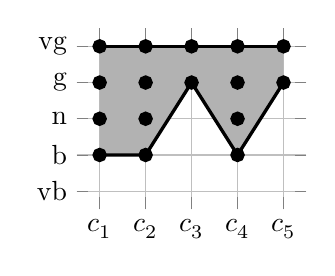
\begin{tikzpicture}
	\begin{axis}[width = 4.5cm, ytick = {-2,-1,0,1,2}, xtick = {1,2,3,4,5}, xmin = 0.5, xmax = 5.500000, ymin = -2.5, ymax = 2.5, axis line style = {draw = none}, xmajorgrids, ymajorgrids, separate axis lines, yticklabels = {vb, b, n, g, vg}, xticklabels = {$c_1$,$c_2$,$c_3$,$c_4$,$c_5$}]
	\addplot[name path = A, black, no markers, solid, very thick]
	coordinates {
		(1,2)
		(2,2)
		(3,2)
		(4,2)
		(5,2)
	};
	\addplot[name path = B, black, no markers, solid, very thick]
	coordinates {
		(1,-1)
		(2,-1)
		(3,1)
		(4,-1)
		(5,1)
	};
	\addplot[name path = C, black, mark = *, only marks, very thick]
	coordinates {
		(1,-1)
		(1,0)
		(1,1)
		(1,2)
		(2,-1)
		(2,0)
		(2,1)
		(2,2)
		(3,1)
		(3,2)
		(4,-1)
		(4,0)
		(4,1)
		(4,2)
		(5,1)
		(5,2)
	};
	\addplot[white!70!black] fill between[of=A and B];
	\end{axis}
	\end{tikzpicture}
	\noindent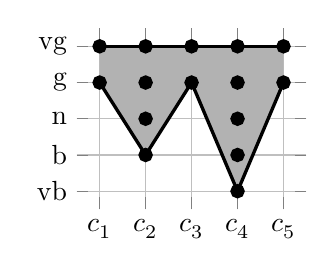
\begin{tikzpicture}
	\begin{axis}[width = 4.5cm, ytick = {-2,-1,0,1,2}, xtick = {1,2,3,4,5}, xmin = 0.5, xmax = 5.500000, ymin = -2.5, ymax = 2.5, axis line style = {draw = none}, xmajorgrids, ymajorgrids, separate axis lines, yticklabels = {vb, b, n, g, vg}, xticklabels = {$c_1$,$c_2$,$c_3$,$c_4$,$c_5$}]
	\addplot[name path = A, black, no markers, solid, very thick]
	coordinates {
		(1,2)
		(2,2)
		(3,2)
		(4,2)
		(5,2)
	};
	\addplot[name path = B, black, no markers, solid, very thick]
	coordinates {
		(1,1)
		(2,-1)
		(3,1)
		(4,-2)
		(5,1)
	};
	\addplot[name path = C, black, mark = *, only marks, very thick]
	coordinates {
		(1,1)
		(1,2)
		(2,-1)
		(2,0)
		(2,1)
		(2,2)
		(3,1)
		(3,2)
		(4,-2)
		(4,-1)
		(4,0)
		(4,1)
		(4,2)
		(5,1)
		(5,2)
	};
	\addplot[white!70!black] fill between[of=A and B];
	\end{axis}
	\end{tikzpicture}
	\noindent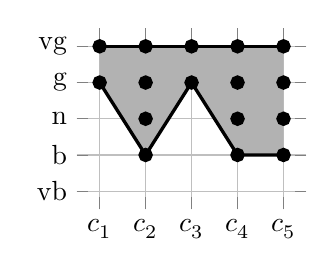
\begin{tikzpicture}
	\begin{axis}[width = 4.5cm, ytick = {-2,-1,0,1,2}, xtick = {1,2,3,4,5}, xmin = 0.5, xmax = 5.500000, ymin = -2.5, ymax = 2.5, axis line style = {draw = none}, xmajorgrids, ymajorgrids, separate axis lines, yticklabels = {vb, b, n, g, vg}, xticklabels = {$c_1$,$c_2$,$c_3$,$c_4$,$c_5$}]
	\addplot[name path = A, black, no markers, solid, very thick]
	coordinates {
		(1,2)
		(2,2)
		(3,2)
		(4,2)
		(5,2)
	};
	\addplot[name path = B, black, no markers, solid, very thick]
	coordinates {
		(1,1)
		(2,-1)
		(3,1)
		(4,-1)
		(5,-1)
	};
	\addplot[name path = C, black, mark = *, only marks, very thick]
	coordinates {
		(1,1)
		(1,2)
		(2,-1)
		(2,0)
		(2,1)
		(2,2)
		(3,1)
		(3,2)
		(4,-1)
		(4,0)
		(4,1)
		(4,2)
		(5,-1)
		(5,0)
		(5,1)
		(5,2)
	};
	\addplot[white!70!black] fill between[of=A and B];
	\end{axis}
	\end{tikzpicture}
	\noindent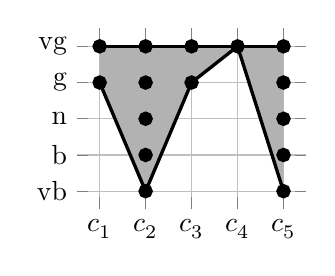
\begin{tikzpicture}
	\begin{axis}[width = 4.5cm, ytick = {-2,-1,0,1,2}, xtick = {1,2,3,4,5}, xmin = 0.5, xmax = 5.500000, ymin = -2.5, ymax = 2.5, axis line style = {draw = none}, xmajorgrids, ymajorgrids, separate axis lines, yticklabels = {vb, b, n, g, vg}, xticklabels = {$c_1$,$c_2$,$c_3$,$c_4$,$c_5$}]
	\addplot[name path = A, black, no markers, solid, very thick]
	coordinates {
		(1,2)
		(2,2)
		(3,2)
		(4,2)
		(5,2)
	};
	\addplot[name path = B, black, no markers, solid, very thick]
	coordinates {
		(1,1)
		(2,-2)
		(3,1)
		(4,2)
		(5,-2)
	};
	\addplot[name path = C, black, mark = *, only marks, very thick]
	coordinates {
		(1,1)
		(1,2)
		(2,-2)
		(2,-1)
		(2,0)
		(2,1)
		(2,2)
		(3,1)
		(3,2)
		(4,2)
		(5,-2)
		(5,-1)
		(5,0)
		(5,1)
		(5,2)
	};
	\addplot[white!70!black] fill between[of=A and B];
	\end{axis}
	\end{tikzpicture}
	
		\vspace{1ex}
		\hrule
		\vspace{1ex}
		
	{\bf Bad Contributors}
	
		\vspace{1ex}
		\hrule
		\vspace{1ex}
	
	\noindent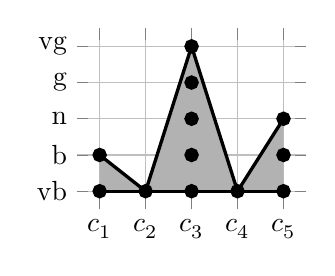
\begin{tikzpicture}
	\begin{axis}[width = 4.5cm, ytick = {-2,-1,0,1,2}, xtick = {1,2,3,4,5}, xmin = 0.5, xmax = 5.500000, ymin = -2.5, ymax = 2.5, axis line style = {draw = none}, xmajorgrids, ymajorgrids, separate axis lines, yticklabels = {vb, b, n, g, vg}, xticklabels = {$c_1$,$c_2$,$c_3$,$c_4$,$c_5$}]
	\addplot[name path = A, black, no markers, solid, very thick]
	coordinates {
		(1,-1)
		(2,-2)
		(3,2)
		(4,-2)
		(5,0)
	};
	\addplot[name path = B, black, no markers, solid, very thick]
	coordinates {
		(1,-2)
		(2,-2)
		(3,-2)
		(4,-2)
		(5,-2)
	};
	\addplot[name path = C, black, mark = *, only marks, very thick]
	coordinates {
		(1,-2)
		(1,-1)
		(2,-2)
		(3,-2)
		(3,-1)
		(3,0)
		(3,1)
		(3,2)
		(4,-2)
		(5,-2)
		(5,-1)
		(5,0)
	};
	\addplot[white!70!black] fill between[of=A and B];
	\end{axis}
	\end{tikzpicture}
	\noindent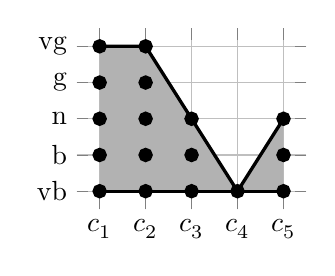
\begin{tikzpicture}
	\begin{axis}[width = 4.5cm, ytick = {-2,-1,0,1,2}, xtick = {1,2,3,4,5}, xmin = 0.5, xmax = 5.500000, ymin = -2.5, ymax = 2.5, axis line style = {draw = none}, xmajorgrids, ymajorgrids, separate axis lines, yticklabels = {vb, b, n, g, vg}, xticklabels = {$c_1$,$c_2$,$c_3$,$c_4$,$c_5$}]
	\addplot[name path = A, black, no markers, solid, very thick]
	coordinates {
		(1,2)
		(2,2)
		(3,0)
		(4,-2)
		(5,0)
	};
	\addplot[name path = B, black, no markers, solid, very thick]
	coordinates {
		(1,-2)
		(2,-2)
		(3,-2)
		(4,-2)
		(5,-2)
	};
	\addplot[name path = C, black, mark = *, only marks, very thick]
	coordinates {
		(1,-2)
		(1,-1)
		(1,0)
		(1,1)
		(1,2)
		(2,-2)
		(2,-1)
		(2,0)
		(2,1)
		(2,2)
		(3,-2)
		(3,-1)
		(3,0)
		(4,-2)
		(5,-2)
		(5,-1)
		(5,0)
	};
	\addplot[white!70!black] fill between[of=A and B];
	\end{axis}
	\end{tikzpicture}
	\noindent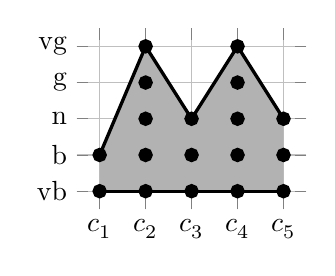
\begin{tikzpicture}
	\begin{axis}[width = 4.5cm, ytick = {-2,-1,0,1,2}, xtick = {1,2,3,4,5}, xmin = 0.5, xmax = 5.500000, ymin = -2.5, ymax = 2.5, axis line style = {draw = none}, xmajorgrids, ymajorgrids, separate axis lines, yticklabels = {vb, b, n, g, vg}, xticklabels = {$c_1$,$c_2$,$c_3$,$c_4$,$c_5$}]
	\addplot[name path = A, black, no markers, solid, very thick]
	coordinates {
		(1,-1)
		(2,2)
		(3,0)
		(4,2)
		(5,0)
	};
	\addplot[name path = B, black, no markers, solid, very thick]
	coordinates {
		(1,-2)
		(2,-2)
		(3,-2)
		(4,-2)
		(5,-2)
	};
	\addplot[name path = C, black, mark = *, only marks, very thick]
	coordinates {
		(1,-2)
		(1,-1)
		(2,-2)
		(2,-1)
		(2,0)
		(2,1)
		(2,2)
		(3,-2)
		(3,-1)
		(3,0)
		(4,-2)
		(4,-1)
		(4,0)
		(4,1)
		(4,2)
		(5,-2)
		(5,-1)
		(5,0)
	};
	\addplot[white!70!black] fill between[of=A and B];
	\end{axis}
	\end{tikzpicture}
	\noindent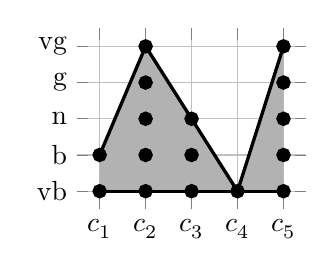
\begin{tikzpicture}
	\begin{axis}[width = 4.5cm, ytick = {-2,-1,0,1,2}, xtick = {1,2,3,4,5}, xmin = 0.5, xmax = 5.500000, ymin = -2.5, ymax = 2.5, axis line style = {draw = none}, xmajorgrids, ymajorgrids, separate axis lines, yticklabels = {vb, b, n, g, vg}, xticklabels = {$c_1$,$c_2$,$c_3$,$c_4$,$c_5$}]
	\addplot[name path = A, black, no markers, solid, very thick]
	coordinates {
		(1,-1)
		(2,2)
		(3,0)
		(4,-2)
		(5,2)
	};
	\addplot[name path = B, black, no markers, solid, very thick]
	coordinates {
		(1,-2)
		(2,-2)
		(3,-2)
		(4,-2)
		(5,-2)
	};
	\addplot[name path = C, black, mark = *, only marks, very thick]
	coordinates {
		(1,-2)
		(1,-1)
		(2,-2)
		(2,-1)
		(2,0)
		(2,1)
		(2,2)
		(3,-2)
		(3,-1)
		(3,0)
		(4,-2)
		(5,-2)
		(5,-1)
		(5,0)
		(5,1)
		(5,2)
	};
	\addplot[white!70!black] fill between[of=A and B];
	\end{axis}
	\end{tikzpicture}
	
	\noindent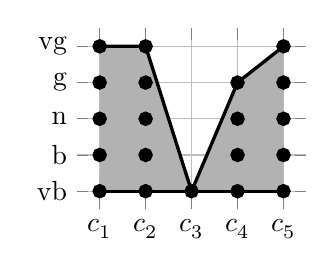
\begin{tikzpicture}
	\begin{axis}[width = 4.5cm, ytick = {-2,-1,0,1,2}, xtick = {1,2,3,4,5}, xmin = 0.5, xmax = 5.500000, ymin = -2.5, ymax = 2.5, axis line style = {draw = none}, xmajorgrids, ymajorgrids, separate axis lines, yticklabels = {vb, b, n, g, vg}, xticklabels = {$c_1$,$c_2$,$c_3$,$c_4$,$c_5$}]
	\addplot[name path = A, black, no markers, solid, very thick]
	coordinates {
		(1,2)
		(2,2)
		(3,-2)
		(4,1)
		(5,2)
	};
	\addplot[name path = B, black, no markers, solid, very thick]
	coordinates {
		(1,-2)
		(2,-2)
		(3,-2)
		(4,-2)
		(5,-2)
	};
	\addplot[name path = C, black, mark = *, only marks, very thick]
	coordinates {
		(1,-2)
		(1,-1)
		(1,0)
		(1,1)
		(1,2)
		(2,-2)
		(2,-1)
		(2,0)
		(2,1)
		(2,2)
		(3,-2)
		(4,-2)
		(4,-1)
		(4,0)
		(4,1)
		(5,-2)
		(5,-1)
		(5,0)
		(5,1)
		(5,2)
	};
	\addplot[white!70!black] fill between[of=A and B];
	\end{axis}
	\end{tikzpicture}
	\noindent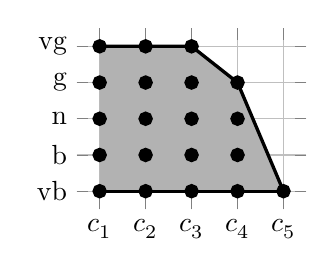
\begin{tikzpicture}
	\begin{axis}[width = 4.5cm, ytick = {-2,-1,0,1,2}, xtick = {1,2,3,4,5}, xmin = 0.5, xmax = 5.500000, ymin = -2.5, ymax = 2.5, axis line style = {draw = none}, xmajorgrids, ymajorgrids, separate axis lines, yticklabels = {vb, b, n, g, vg}, xticklabels = {$c_1$,$c_2$,$c_3$,$c_4$,$c_5$}]
	\addplot[name path = A, black, no markers, solid, very thick]
	coordinates {
		(1,2)
		(2,2)
		(3,2)
		(4,1)
		(5,-2)
	};
	\addplot[name path = B, black, no markers, solid, very thick]
	coordinates {
		(1,-2)
		(2,-2)
		(3,-2)
		(4,-2)
		(5,-2)
	};
	\addplot[name path = C, black, mark = *, only marks, very thick]
	coordinates {
		(1,-2)
		(1,-1)
		(1,0)
		(1,1)
		(1,2)
		(2,-2)
		(2,-1)
		(2,0)
		(2,1)
		(2,2)
		(3,-2)
		(3,-1)
		(3,0)
		(3,1)
		(3,2)
		(4,-2)
		(4,-1)
		(4,0)
		(4,1)
		(5,-2)
	};
	\addplot[white!70!black] fill between[of=A and B];
	\end{axis}
	\end{tikzpicture}
	
		\vspace{1ex}
		\hrule
	
    \caption{Assignment rules for good and bad contributors from the perspective of \GJ.}\label{fig:ex1-rules-reduced}
\end{figure}

We explained the interpretation of the rules verbally to 
\GJ, who validated the illustrated rules without making any changes to them.

\subsubsection{Inferring the preference model of \DB}

We started with the same set of 25 alternatives initially used by \GJ to better illustrate the differences between the two DMs. \DB's assignments are shown in Table~\ref{tab:ex2-data1}. During this process one author was also on hand to record any rationale expressed by \DB.

\begin{table}
\caption{The initial set of contributor profiles and their assignment by \DB;}\label{tab:ex2-data1}
\setlength{\tabcolsep}{4pt}
\tabulinesep=2pt
\begin{minipage}[t]{.49\textwidth}
\vspace{0pt}

\centering

\begin{tabu}{c|ccccc|c}
Profile& \multicolumn{5}{c|}{Criteria} & Assigned\\
number& $c_1$ & $c_2$ & $c_3$ & $c_4$ & $c_5$ & category \\\hline
1 &vg & g &vb &vg & n & Good\\
2 & b &vg & n &vb & n & Bad\\
3 & b & b & b & b & g & Bad\\
4 & b & b &vb &vg & n & Bad\\
5 & g &vb &vg & b & b & Neutral\\
6 &vg & g &vg & n &vg & Good\\
7 & g & n & b & n &vg & Good\\
8 & n & n & g & b & g & Neutral\\
9 & n &vg & n & g & b & Good\\
10&vb & g &vg &vb & b & Bad\\
11& g & g & g &vb &vg & Good\\
12& n & g & g &vb & g & Good\\
13& g & g & n & n &vb & Good
\end{tabu}
\end{minipage}
\hfill
\begin{minipage}[t]{.49\textwidth}
\vspace{0pt}

\centering

\begin{tabu}{c|ccccc|c}
Profile& \multicolumn{5}{c|}{Criteria} & Assigned\\
number& $c_1$ & $c_2$ & $c_3$ & $c_4$ & $c_5$ & category \\\hline
14&vg & n &vb & b & g & Good\\
15& n & b & b &vb & n & Bad\\
16& b &vg & g &vg &vb & Neutral\\
17& n & b & n & g & n & Neutral\\
18&vg &vb &vg & g & b & Neutral\\
19&vg &vb & n & n &vb & Neutral\\
20&vb &vg &vg & b &vg & Bad\\
21&vb & n &vb & n &vb & Bad\\
22&vb & b &vb &vg & g & Bad\\
23&vb &vb & g & g &vg & Bad\\
24& g &vb & b & g &vb & Neutral\\
25& b & n & b &vg & b & Bad
\end{tabu}
\end{minipage}
\end{table}

We tried to fit the data with an MR-Sort model and found that at most 24 of the 25 assignment examples could be captured with this type of model. Therefore we provided the DM with the possible sets of alternatives shown in Table~\ref{tab:ex2-altassig1}.

\begin{table}
\caption{The alternative assignments for an MR-Sort model within the first iteration of the inference protocol for \DB.}\label{tab:ex2-altassig1}
\setlength{\tabcolsep}{4pt}
\tabulinesep=2pt

\centering

\begin{tabu}{cc|ccccc|cc}
&Profile& \multicolumn{5}{c|}{Criteria} & \multicolumn{2}{c}{Category} \\
%&number& $c_1$ & $c_2$ & $c_3$ & $c_4$ & $c_5$ & \multicolumn{1}{c}{CM} & \multicolumn{1}{c}{MR-Sort} \\\hline
&number& $c_1$ & $c_2$ & $c_3$ & $c_4$ & $c_5$ & \multicolumn{1}{c}{original} & \multicolumn{1}{c}{alternative} \\\hline
First set& 8 &  n & n & g & b & g &  Neutral & Good \\[2pt]
Second set& 14 & vg & n & vb & b & g &  Good & Neutral
\end{tabu}
% \begin{tabular}{cccccc|cc}
% Profile& \multicolumn{5}{c}{Criteria} & \multicolumn{2}{|c}{Category} \\
% number& $c_1$ & $c_2$ & $c_3$ & $c_4$ & $c_5$ & \multicolumn{1}{c}{original} & \multicolumn{1}{c}{alternative} \\\hline
% 8 &neutral & neutral &    good &     bad &    good & Neutral & Good \\\hline
% 14 &v. good & neutral &  v. bad &     bad &    good & Good & Neutral \\        
% \end{tabular}
\end{table}

\DB had already verbally expressed hesitation in assigning the eigth profile, and therefore agreed to change his assignment. The resulting MR-Sort model is presented in Figure~\ref{fig:ex2-model1}.

\begin{figure}
\centering

\begin{minipage}[c]{0.4\columnwidth}
\vspace{0pt}
\begin{tikzpicture}
\begin{axis}[title ={Bad-Neutral}, height=\textwidth,width=\textwidth, xmin = 0.5, xmax = 5.5, ymin = -2.5, ymax = 2.5, every axis x label/.style={at={(ticklabel* cs:0.97)},anchor=south},xtick={1,2,3,4,5}, xticklabels={$c_1$,$c_2$,$c_3$,$c_4$,$c_5$}, ytick={-2,-1,0,1,2}, xmajorgrids = true, axis line style = { draw = none }, yticklabels = {vb, b, n, g, vg}, ymajorgrids = true]
\addplot[name path=T]
coordinates {
	(1,3)
	(2,3)
	(3,3)
	(4,3)
	(5,3)
};
\addplot[name path=B]
coordinates {
	(1,-3)
	(2,-3)
	(3,-3)
	(4,-3)
	(5,-3)
};
\addplot[name path=P, black, solid, mark = *]
coordinates {
	(1,-0.5)
	(2,-0.5)
	(3,-0.5)
	(4,-0.5)
	(5,-2)
};
\end{axis}
\end{tikzpicture}
\end{minipage}
\begin{minipage}[c]{0.4\columnwidth}
\vspace{0pt}

\begin{tikzpicture}
\begin{axis}[title ={Neutral-Good}, height=\textwidth,width=\textwidth, xmin = 0.5, xmax = 5.5, ymin = -2.5, ymax = 2.5, every axis x label/.style={at={(ticklabel* cs:0.97)},anchor=south},xtick={1,2,3,4,5}, xticklabels={$c_1$,$c_2$,$c_3$,$c_4$,$c_5$}, ytick={-2,-1,0,1,2}, xmajorgrids = true, axis line style = { draw = none }, yticklabels = {vb, b, n, g, vg}, ymajorgrids = true]
\addplot[name path=T]
coordinates {
	(1,3)
	(2,3)
	(3,3)
	(4,3)
	(5,3)
};
\addplot[name path=B]
coordinates {
	(1,-3)
	(2,-3)
	(3,-3)
	(4,-3)
	(5,-3)
};
\addplot[name path=P, black, solid, mark = *]
coordinates {
	(1,-0.5)
	(2,-0.5)
	(3,-0.5)
	(4,0.5)
	(5,0.5)
};
\end{axis}
\end{tikzpicture}
\end{minipage}
\begin{minipage}[c]{0.07\columnwidth}
\vspace{0pt}

\begin{tabular}{c|c}
$\lambda$ & 0.6 \\\hline
$c_1$ & 0.40 \\
$c_2$ & 0.15 \\
$c_3$ & 0.15 \\
$c_4$ & 0.15 \\
$c_5$ & 0.15 \\
\end{tabular}
\end{minipage}
\caption{First preference model of \DB (MR-Sort).}\label{fig:ex2-model1}
\end{figure}

We continued with a second iteration by generating an additional 10 profiles based on the existing model. This new set was presented to \DB, who assigned them as shown in Table~\ref{tab:ex2-data2}.

\begin{table}
\caption{The second set of contributor profiles and their assignment by \DB.}\label{tab:ex2-data2}
\setlength{\tabcolsep}{4pt}
\tabulinesep=2pt
\begin{minipage}[t]{.49\textwidth}
\vspace{0pt}

\centering

\begin{tabu}{c|ccccc|c}
Profile& \multicolumn{5}{c|}{Criteria} & Assigned\\
number& $c_1$ & $c_2$ & $c_3$ & $c_4$ & $c_5$ & category \\\hline
26 &b & b &b &vg & vg & Bad\\
27 &vb & n & g &n & g & Bad\\
28 &vg & b & n & b & n & Neutral\\
29 &n &n & vb & vb & g & Neutral\\
30 &b &b & vg & b & vg & Bad
\end{tabu}
\end{minipage}
\hfill
\begin{minipage}[t]{.49\textwidth}
\vspace{0pt}

\centering

\begin{tabu}{c|ccccc|c}
Profile& \multicolumn{5}{c|}{Criteria} & Assigned\\
number& $c_1$ & $c_2$ & $c_3$ & $c_4$ & $c_5$ & category \\\hline
31&n & n &g &vb & vb & Neutral\\
32&n & vb & n &vb & vb & Bad\\
33&vb &n &n &n &vb & Bad\\
34&n &n &vb &n &vb & Bad\\
35&n &vb & vb &n & g & Neutral
\end{tabu}
\end{minipage}

% \begin{tabular}{cccccc||c}
% Profile& \multicolumn{5}{c}{Criteria} & \multicolumn{1}{c}{Category assignment}\\
% 26& bad & bad & bad & v. good & v. good & Bad \\\hline
% 27& v. bad & neutral & good & neutral & good & Bad \\\hline
% 28& v. good & bad & neutral & bad & neutral & Neutral \\\hline
% 29& neutral & neutral & v. bad & v. bad & good & Neutral \\\hline
% 30& bad & bad & v. good & bad & v. good & Bad \\\hline
% 31& neutral & neutral & good & v. bad & v. bad & Neutral \\\hline
% 32& neutral & v. bad & neutral & v. bad & v. bad & Bad \\\hline
% 33& v. bad & neutral & neutral & neutral & v. bad & Bad \\\hline
% 34& neutral & neutral & v. bad & neutral & v. bad & Bad \\\hline
% 35& neutral & v. bad & v. bad & neutral & good & Neutral \\\hline
% \end{tabular}
\end{table}

We combined the initial 25 profiles with the 10 new profiles and checked their fit with an MR-Sort model. As only 33 out of the 35 profiles could be represented by this model, we proceeded to determine if the DM would accept adapting a minimal number of his assignments. Only one set of profile changes would make this possible. This option is shown in Table~\ref{tab:ex2-altassig2}.

\begin{table}
\caption{The alternative assignments for an MR-Sort model within the second iteration of the inference protocol for \DB.}\label{tab:ex2-altassig2}
\setlength{\tabcolsep}{4pt}
\tabulinesep=2pt

\centering

\begin{tabu}{cc|ccccc|cc}
&Profile& \multicolumn{5}{c|}{Criteria} & \multicolumn{2}{c}{Category} \\
%&number& $c_1$ & $c_2$ & $c_3$ & $c_4$ & $c_5$ & \multicolumn{1}{c}{CM} & \multicolumn{1}{c}{MR-Sort} \\\hline
&number& $c_1$ & $c_2$ & $c_3$ & $c_4$ & $c_5$ & \multicolumn{1}{c}{original} & \multicolumn{1}{c}{alternative} \\\hline
\multirow{2}{*}{First set}& 16 &  b & vg & g & vg & vb &  Neutral & Bad \\
& 34 &  n & n & vb & n & vb &  Bad & Good \\
\end{tabu}
% \begin{tabular}{ccccccc|cc}
% &Profile& \multicolumn{5}{c}{Criteria} & \multicolumn{2}{|c}{Category} \\
% &number& $c_1$ & $c_2$ & $c_3$ & $c_4$ & $c_5$ & \multicolumn{1}{c}{original} & \multicolumn{1}{c}{alternative} \\\hline
% \multirow{2}{*}{First set}& 16&    bad & v. good &    good & v. good &  v. bad &  Neutral & Bad \\
% & 34& neutral & neutral & v. bad & neutral & v. bad &  Bad & Good \\
% \end{tabular}
\end{table}

\DB expressed a willingness to change the assignment of the first profile from this set. However, the change in assignment for the second profile was too drastic. Therefore we looked at a more complicated model, in particular an MR-Sort with vetoes or an MR-Sort with dictators, could describe the assignments. Both of these models were also unable fit the data completely, but the model with dictators required two profiles to be changed, whereas the model with vetoes only needed one profile change. Therefore we focused on the MR-Sort with vetoes. The possible profile changes are found in Table~\ref{tab:ex2-altassig3}.

\begin{table}
\caption{The alternative assignments for an MR-Sort model with vetoes within the second iteration of the inference protocol for \DB.}\label{tab:ex2-altassig3}
\setlength{\tabcolsep}{4pt}
\tabulinesep=2pt

\centering

\begin{tabu}{cc|ccccc|cc}
&Profile& \multicolumn{5}{c|}{Criteria} & \multicolumn{2}{c}{Category} \\
%&number& $c_1$ & $c_2$ & $c_3$ & $c_4$ & $c_5$ & \multicolumn{1}{c}{CM} & \multicolumn{1}{c}{MR-Sort} \\\hline
&number& $c_1$ & $c_2$ & $c_3$ & $c_4$ & $c_5$ & \multicolumn{1}{c}{original} & \multicolumn{1}{c}{alternative} \\\hline
First set& 16 &  b & vg & g & vg & vb &  Neutral & Bad \\[2pt]
Second set& 32 & n & vb & n & vb & vb &  Bad & Neutral \\[2pt]
Third set& 34 &  n & n & vb & n & vb &  Bad & Neutral
\end{tabu}
% \begin{tabular}{cccccc|cc}
% Profile& \multicolumn{5}{c}{Criteria} & \multicolumn{2}{|c}{Category} \\
% number& $c_1$ & $c_2$ & $c_3$ & $c_4$ & $c_5$ & \multicolumn{1}{c}{original} & \multicolumn{1}{c}{alternative} \\\hline
%  16&    bad & v. good &    good & v. good &  v. bad &  Neutral & Bad \\\hline
%  32& neutral & v. bad & neutral & v. bad & v. bad &  Bad & Neutral \\\hline
%  34& neutral & neutral & v. bad & neutral & v. bad &  Bad & Neutral \\
% \end{tabular}
\end{table}


As the DM had previously expressed a hesitation on the assignment of profile 16, he quickly agreed to the proposed changed. The model that reflects all assignments at the end of the second iteration is depicted in Figure~\ref{fig:ex2-model2}.

\begin{figure}
\centering

\begin{minipage}[c]{0.4\columnwidth}
\vspace{0pt}
\begin{tikzpicture}
\begin{axis}[title ={Bad-Neutral}, height=\textwidth,width=\textwidth, xmin = 0.5, xmax = 5.5, ymin = -2.5, ymax = 2.5, every axis x label/.style={at={(ticklabel* cs:0.97)},anchor=south},xtick={1,2,3,4,5}, xticklabels={$c_1$,$c_2$,$c_3$,$c_4$,$c_5$}, ytick={-2,-1,0,1,2}, xmajorgrids = true, axis line style = { draw = none }, yticklabels = {vb, b, n, g, vg}, ymajorgrids = true]
\addplot[name path=T]
coordinates {
	(1,3)
	(2,3)
	(3,3)
	(4,3)
	(5,3)
};
\addplot[name path=B]
coordinates {
	(1,-3)
	(2,-3)
	(3,-3)
	(4,-3)
	(5,-3)
};
\addplot[name path=P, black, solid, mark = *]
coordinates {
	(1,0.5)
	(2,-1.5)
	(3,-0.5)
	(4,-2)
	(5,0.5)
};
\addplot[name path=V]
coordinates {
	(0,-1)
	(1,-3)
	(2,-3)
	(3,-3)
	(4,-3)
	(5,-3)
};
\addplot[black] fill between[of=V and B];
\end{axis}
\end{tikzpicture}
\end{minipage}
\begin{minipage}[c]{0.4\columnwidth}
\vspace{0pt}

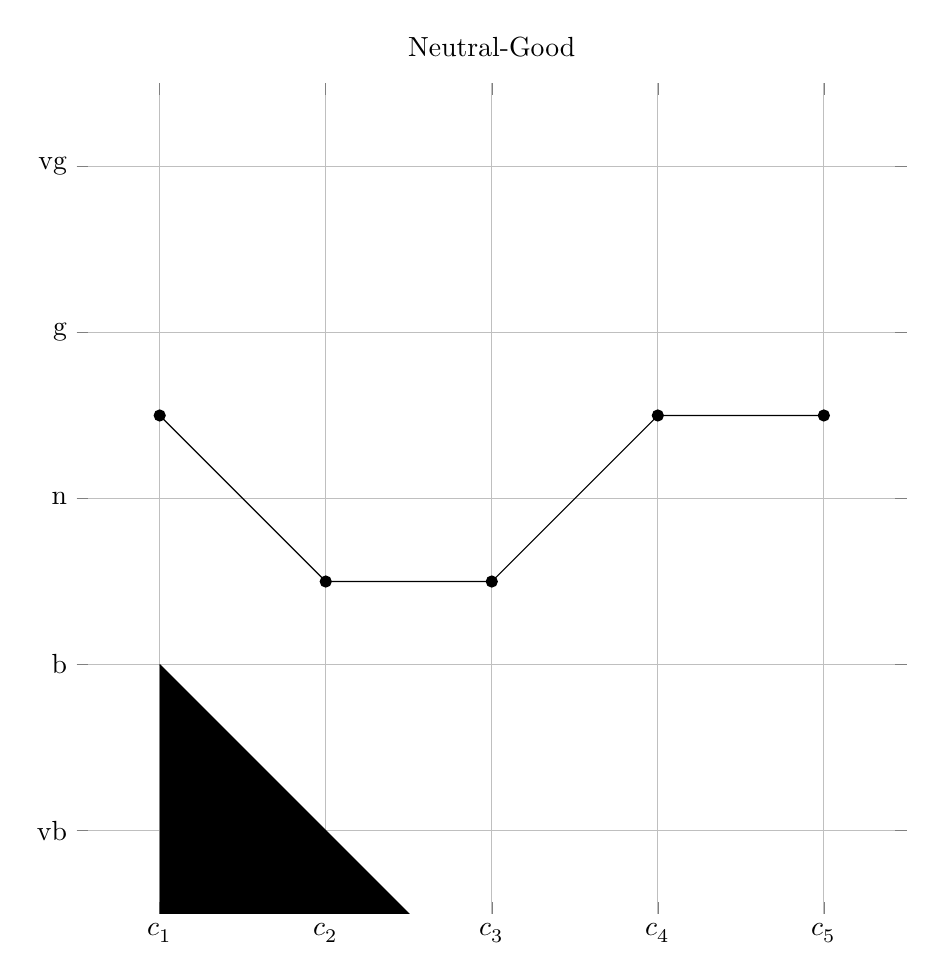
\begin{tikzpicture}
\begin{axis}[title ={Neutral-Good}, height=\textwidth,width=\textwidth, xmin = 0.5, xmax = 5.5, ymin = -2.5, ymax = 2.5, every axis x label/.style={at={(ticklabel* cs:0.97)},anchor=south},xtick={1,2,3,4,5}, xticklabels={$c_1$,$c_2$,$c_3$,$c_4$,$c_5$}, ytick={-2,-1,0,1,2}, xmajorgrids = true, axis line style = { draw = none }, yticklabels = {vb, b, n, g, vg}, ymajorgrids = true]
\addplot[name path=T]
coordinates {
	(1,3)
	(2,3)
	(3,3)
	(4,3)
	(5,3)
};
\addplot[name path=B]
coordinates {
	(1,-3)
	(2,-3)
	(3,-3)
	(4,-3)
	(5,-3)
};
\addplot[name path=P, black, solid, mark = *]
coordinates {
	(1,0.5)
	(2,-0.5)
	(3,-0.5)
	(4,0.5)
	(5,0.5)
};
\addplot[name path=V]
coordinates {
	(1,-1)
	(2,-2)
	(3,-3)
	(4,-3)
	(5,-3)
};
\addplot[black] fill between[of=V and B];
\end{axis}
\end{tikzpicture}
\end{minipage}
\begin{minipage}[c]{0.07\columnwidth}
\vspace{0pt}

\begin{tabular}{c|c}
$\lambda$ & 0.5 \\\hline
$c_1$ & 0.16733 \\
$c_2$ & 0.16733 \\
$c_3$ & 0.16733 \\
$c_4$ & 0.33267 \\
$c_5$ & 0.16733
\end{tabular}
\end{minipage}

\caption{Second preference model of \DB (MR-Sort with vetoes).}\label{fig:ex2-model2}
\end{figure}

The model appeared to further illustrate the existence of vetoes on the first two criteria, which we had already posited from the reasoning the DM expressed in the assignment interview. \DB agreed to continue with another iteration of the protocol.

We generated an additional set of 10 profiles, which were assigned as illustrated in Table~\ref{tab:ex2-data3}.

\begin{table}
\caption{The third set of contributor profiles and their assignment by \DB.}\label{tab:ex2-data3}
\setlength{\tabcolsep}{4pt}
\tabulinesep=2pt
\begin{minipage}[t]{.49\textwidth}
\vspace{0pt}

\centering

\begin{tabu}{c|ccccc|c}
Profile& \multicolumn{5}{c|}{Criteria} & Assigned\\
number& $c_1$ & $c_2$ & $c_3$ & $c_4$ & $c_5$ & category \\\hline
36 &n & vb &vb &vb & g & Neutral\\
37 &n & g & n &vb & g & Neutral\\
38 &vg & vb & vg & vg & vg & Good\\
39 &b &vg & vg & vg & vg & Neutral\\
40 &n &n & b & vg & vg & Neutral
\end{tabu}
\end{minipage}
\hfill
\begin{minipage}[t]{.49\textwidth}
\vspace{0pt}

\centering

\begin{tabu}{c|ccccc|c}
Profile& \multicolumn{5}{c|}{Criteria} & Assigned\\
number& $c_1$ & $c_2$ & $c_3$ & $c_4$ & $c_5$ & category \\\hline
41&g & g &n &vb & vb & Good\\
42&n & vb & b &vg & vg & Neutral\\
43&g &b &vb &vb &vb & Neutral\\
44&n &b &n &vb &vb & Neutral\\
45&vg &vb & b &vg & n & Good
\end{tabu}
\end{minipage}
% \begin{tabular}{cccccc||c}
% Profile& \multicolumn{5}{c}{Criteria} & \multicolumn{1}{c}{Category assignment}\\
% 36 & neutral & v. bad & v. bad & v. bad & good & Neutral \\\hline
% 37 & neutral & good & neutral & v. bad & good & Neutral \\\hline
% 38 & v. good & v. bad & v. good & v. good & v. good & Good \\\hline
% 39 & bad & v. good & v. good & v. good & v. good & Neutral \\\hline
% 40 & neutral & neutral & bad & v. good & v. good & Neutral \\\hline
% 41 & good & good & neutral & v. bad & v. bad & Good \\\hline
% 42 & neutral & v. bad & bad & v. good & v. good & Neutral \\\hline
% 43 & good & bad & v. bad & v. bad & v. bad & Neutral \\\hline
% 44 & neutral & bad & neutral & v. bad & v. bad & Neutral \\\hline
% 45 & v. good & v. bad & bad & v. good & neutral & Good \\\hline
% \end{tabular}
\end{table}

After adding the 10 new profiles and their assignments to the existing ones, we found that an MR-Sort model with vetoes was not able to represent all of these assignments and that at least three profile assignments needed to be altered to allow for this type of model to be used. These sets are presented in Table~\ref{tab:ex2-altassig4}.

\begin{table}
\caption{The alternative assignments for an MR-Sort model with vetoes within the third iteration of the inference protocol for \DB.}\label{tab:ex2-altassig4}
\setlength{\tabcolsep}{4pt}
\tabulinesep=2pt

\centering

\begin{tabu}{cc|ccccc|cc}
&Profile& \multicolumn{5}{c|}{Criteria} & \multicolumn{2}{c}{Category} \\
%&number& $c_1$ & $c_2$ & $c_3$ & $c_4$ & $c_5$ & \multicolumn{1}{c}{CM} & \multicolumn{1}{c}{MR-Sort} \\\hline
&number& $c_1$ & $c_2$ & $c_3$ & $c_4$ & $c_5$ & \multicolumn{1}{c}{original} & \multicolumn{1}{c}{alternative} \\\hline
\multirow{3}{*}{First set}& 9 & n & vg & n & g & b &  Bad & Neutral \\
& 32 & n & vb & n & vb & vb &  Bad & Neutral \\
& 39 & b & vg & vg & vg & vg &  Neutral & Bad \\[2pt]
\multirow{3}{*}{Second set}& 9 & n & vg & n & g & b &  Bad & Neutral \\
& 12 & n & vg & g & vb & g &  Good & Neutral \\
& 39 & b & vg & vg & vg & vg &  Neutral & Bad \\[2pt]
\multirow{3}{*}{Third set}& 38 & vg & vb & vg & vg & vg &  Good & Neutral \\
& 39 & b & vg & vg & vg & vg &  Neutral & Bad \\
& 45 & vg & vb & b & vg & n &  Good & Neutral
\end{tabu}
% \begin{tabular}{ccccccc|cc}
% &Profile& \multicolumn{5}{c}{Criteria} & \multicolumn{2}{|c}{Category} \\
% &number& $c_1$ & $c_2$ & $c_3$ & $c_4$ & $c_5$ & \multicolumn{1}{c}{original} & \multicolumn{1}{c}{alternative} \\\hline
% \multirow{3}{*}{First set}&9 &neutral & v. good & neutral &    good &     bad &  Good & Neutral \\
% &32& neutral & v. bad & neutral & v. bad & v. bad & Bad & Neutral \\
% &39 & bad & v. good & v. good & v. good & v. good & Neutral & Bad \\\hline

% \multirow{3}{*}{Second set}&9 &neutral & v. good & neutral &    good &     bad &  Good & Neutral \\
% &12&neutral & v. good &    good &  v. bad &    good & Good & Neutral \\
% &39 & bad & v. good & v. good & v. good & v. good & Neutral & Bad \\\hline
         
% \multirow{3}{*}{Third set}&38 & v. good & v. bad & v. good & v. good & v. good &  Good & Neutral \\
% &39 & bad & v. good & v. good & v. good & v. good & Neutral & Bad \\
% &45 & v. good & v. bad & bad & v. good & neutral & Good & Neutral \\\hline
% \end{tabular}
\end{table}

As profile 39 appeared in all three sets, we began with asking \DB if he hesitated in assigning this profile. As the answer was negative, we considered a more complex model. An MR-Sort model with veto weakened by a dictator was able to fully reflect all of the DM's assignments. Figure~\ref{fig:ex2-model3} presents this model.

\begin{figure}
\centering

\begin{minipage}[c]{0.4\columnwidth}
\vspace{0pt}
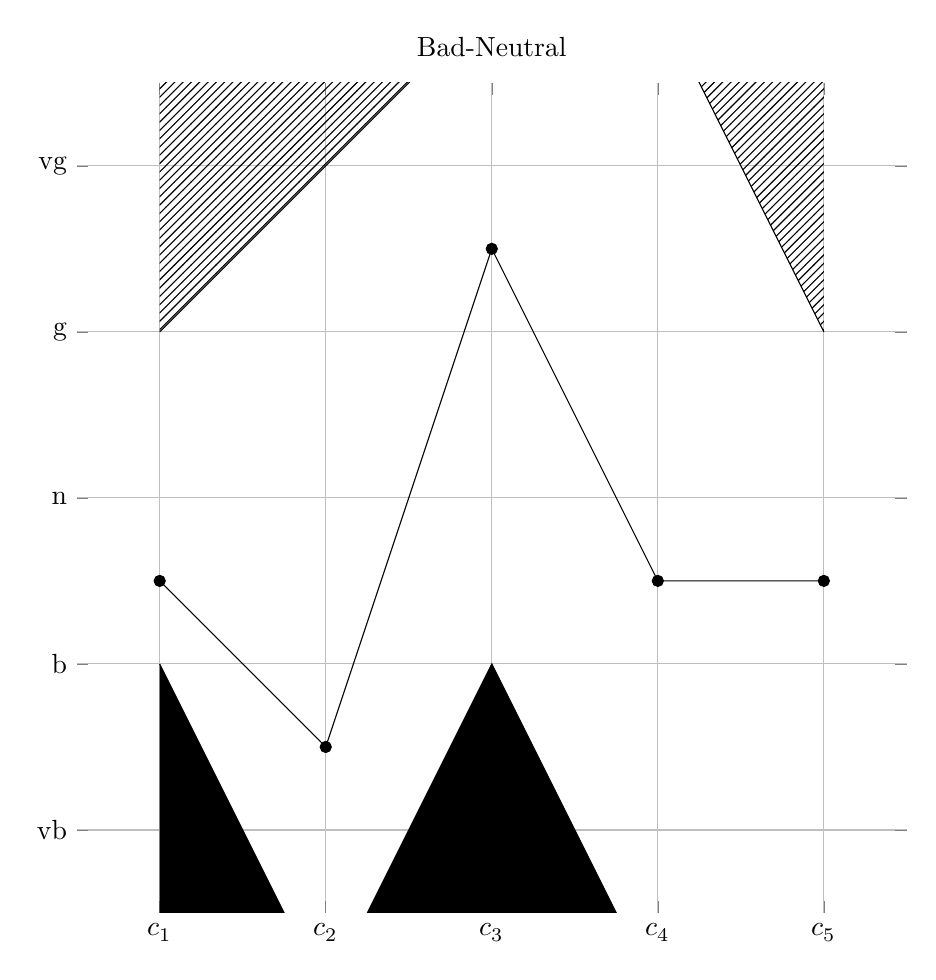
\begin{tikzpicture}
\begin{axis}[title ={Bad-Neutral}, height=\textwidth,width=\textwidth, xmin = 0.5, xmax = 5.5, ymin = -2.5, ymax = 2.5, every axis x label/.style={at={(ticklabel* cs:0.97)},anchor=south},xtick={1,2,3,4,5}, xticklabels={$c_1$,$c_2$,$c_3$,$c_4$,$c_5$}, ytick={-2,-1,0,1,2}, xmajorgrids = true, axis line style = { draw = none }, yticklabels = {vb, b, n, g, vg}, ymajorgrids = true]
\addplot[name path=T]
coordinates {
	(1,3)
	(2,3)
	(3,3)
	(4,3)
	(5,3)
};
\addplot[name path=B]
coordinates {
	(1,-3)
	(2,-3)
	(3,-3)
	(4,-3)
	(5,-3)
};
\addplot[name path=P, black, solid, mark = *]
coordinates {
	(1,-0.5)
	(2,-1.5)
	(3,1.5)
	(4,-0.5)
	(5,-0.5)
};
\addplot[name path=V]
coordinates {
	(1,-1)
	(2,-3)
	(3,-1)
	(4,-3)
	(5,-3)
};
\addplot[name path=D]
coordinates {
	(1,1)
	(2,2)
	(3,3)
	(4,3)
	(5,1)
};
\addplot[black] fill between[of=V and B];
\addplot[pattern = north east lines] fill between[of=D and T];
\end{axis}
\end{tikzpicture}
\end{minipage}
\begin{minipage}[c]{0.4\columnwidth}
\vspace{0pt}

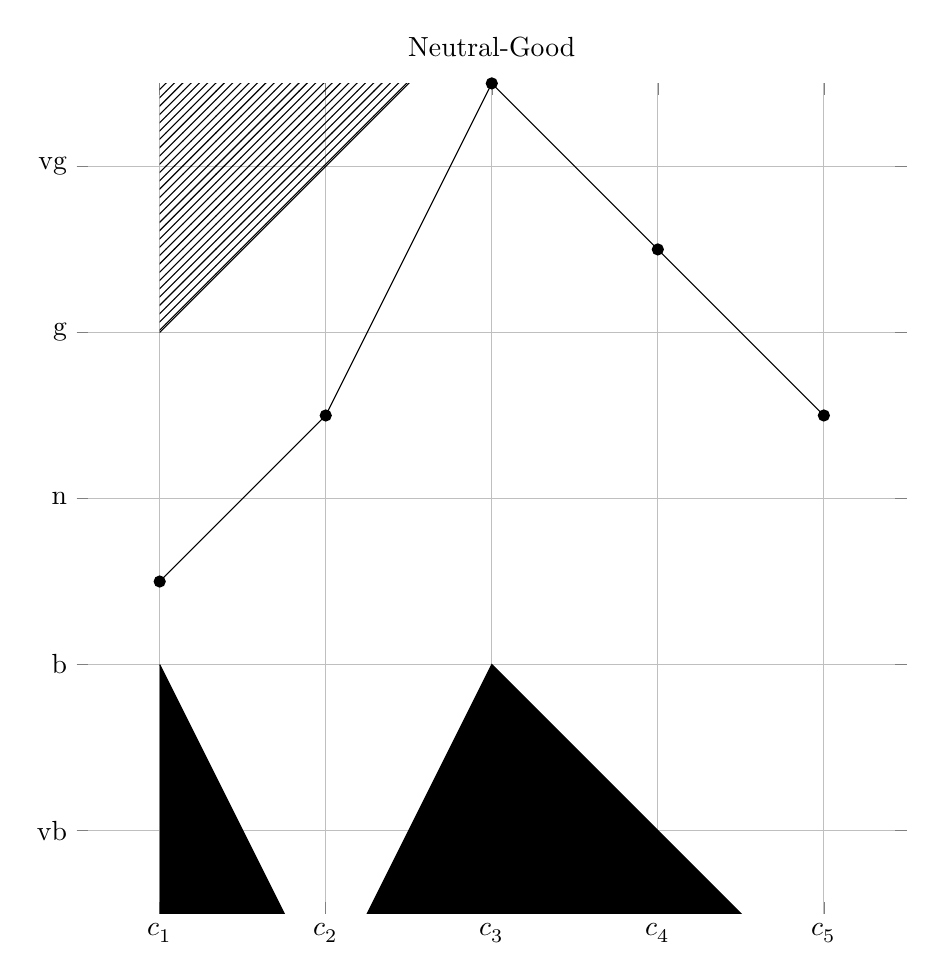
\begin{tikzpicture}
\begin{axis}[title ={Neutral-Good}, height=\textwidth,width=\textwidth, xmin = 0.5, xmax = 5.5, ymin = -2.5, ymax = 2.5, every axis x label/.style={at={(ticklabel* cs:0.97)},anchor=south},xtick={1,2,3,4,5}, xticklabels={$c_1$,$c_2$,$c_3$,$c_4$,$c_5$}, ytick={-2,-1,0,1,2}, xmajorgrids = true, axis line style = { draw = none }, yticklabels = {vb, b, n, g, vg}, ymajorgrids = true]
\addplot[name path=T]
coordinates {
	(1,3)
	(2,3)
	(3,3)
	(4,3)
	(5,3)
};
\addplot[name path=B]
coordinates {
	(1,-3)
	(2,-3)
	(3,-3)
	(4,-3)
	(5,-3)
};
\addplot[name path=P, black, solid, mark = *]
coordinates {
	(1,-0.5)
	(2,0.5)
	(3,2.5)
	(4,1.5)
	(5,0.5)
};
\addplot[name path=V]
coordinates {
	(1,-1)
	(2,-3)
	(3,-1)
	(4,-2)
	(5,-3)
};
\addplot[name path=D]
coordinates {
	(1,1)
	(2,2)
	(3,3)
	(4,3)
	(5,3)
};
\addplot[black] fill between[of=V and B];
\addplot[pattern = north east lines] fill between[of=D and T];
\end{axis}
\end{tikzpicture}
\end{minipage}
\begin{minipage}[c]{0.07\columnwidth}
\vspace{0pt}

\begin{tabular}{c|c}
$\lambda$ & 0.55 \\\hline
$c_1$ & 0.40 \\
$c_2$ & 0.15 \\
$c_3$ & 0.15 \\
$c_4$ & 0.15 \\
$c_5$ & 0.15
\end{tabular}
\end{minipage}

\caption{Third preference model of \DB (MR-Sort with vetoes weakened by dictators).}\label{fig:ex2-model3}
\end{figure}

At this point, we might have constructed a total of 27 new profiles in order to refine the model parameters. The DM, however, expressed an interest in seeing the model, which, after three iterations, already reflected a large portion of his perspective. A set of rules were generated from the model, as shown in Figure~\ref{fig:ex2-rules-reduced1}, and we explained the implications in an interview with \DB.

\begin{figure}
	\centering
	
		\hrule
		\vspace{1ex}
	
	{\bf Good Contributors}
	
		\vspace{1ex}
		\hrule
		\vspace{1ex}

\noindent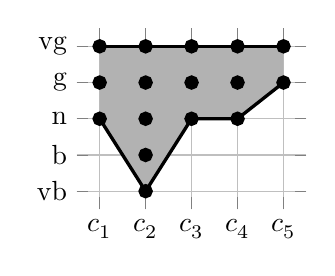
\begin{tikzpicture}
\begin{axis}[width = 4.5cm, ytick = {-2,-1,0,1,2}, xtick = {1,2,3,4,5}, xmin = 0.5, xmax = 5.500000, ymin = -2.5, ymax = 2.5, axis line style = {draw = none}, xmajorgrids, ymajorgrids, separate axis lines, yticklabels = {vb, b, n, g, vg}, xticklabels = {$c_1$,$c_2$,$c_3$,$c_4$,$c_5$}]
\addplot[name path = A, black, no markers, solid, very thick]
coordinates {
	(1,2)
	(2,2)
	(3,2)
	(4,2)
	(5,2)
};
\addplot[name path = B, black, no markers, solid, very thick]
coordinates {
	(1,0)
	(2,-2)
	(3,0)
	(4,0)
	(5,1)
};
\addplot[name path = C, black, mark = *, only marks, very thick]
coordinates {
	(1,0)
	(1,1)
	(1,2)
	(2,-2)
	(2,-1)
	(2,0)
	(2,1)
	(2,2)
	(3,0)
	(3,1)
	(3,2)
	(4,0)
	(4,1)
	(4,2)
	(5,1)
	(5,2)
};
\addplot[white!70!black] fill between[of=A and B];
\end{axis}
\end{tikzpicture}
\noindent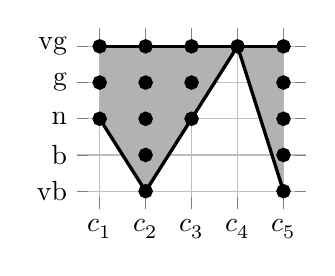
\begin{tikzpicture}
\begin{axis}[width = 4.5cm, ytick = {-2,-1,0,1,2}, xtick = {1,2,3,4,5}, xmin = 0.5, xmax = 5.500000, ymin = -2.5, ymax = 2.5, axis line style = {draw = none}, xmajorgrids, ymajorgrids, separate axis lines, yticklabels = {vb, b, n, g, vg}, xticklabels = {$c_1$,$c_2$,$c_3$,$c_4$,$c_5$}]
\addplot[name path = A, black, no markers, solid, very thick]
coordinates {
	(1,2)
	(2,2)
	(3,2)
	(4,2)
	(5,2)
};
\addplot[name path = B, black, no markers, solid, very thick]
coordinates {
	(1,0)
	(2,-2)
	(3,0)
	(4,2)
	(5,-2)
};
\addplot[name path = C, black, mark = *, only marks, very thick]
coordinates {
	(1,0)
	(1,1)
	(1,2)
	(2,-2)
	(2,-1)
	(2,0)
	(2,1)
	(2,2)
	(3,0)
	(3,1)
	(3,2)
	(4,2)
	(5,-2)
	(5,-1)
	(5,0)
	(5,1)
	(5,2)
};
\addplot[white!70!black] fill between[of=A and B];
\end{axis}
\end{tikzpicture}
\noindent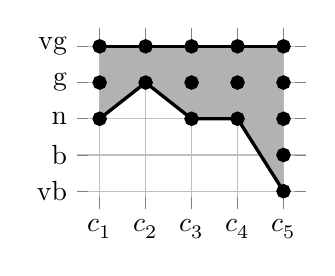
\begin{tikzpicture}
\begin{axis}[width = 4.5cm, ytick = {-2,-1,0,1,2}, xtick = {1,2,3,4,5}, xmin = 0.5, xmax = 5.500000, ymin = -2.5, ymax = 2.5, axis line style = {draw = none}, xmajorgrids, ymajorgrids, separate axis lines, yticklabels = {vb, b, n, g, vg}, xticklabels = {$c_1$,$c_2$,$c_3$,$c_4$,$c_5$}]
\addplot[name path = A, black, no markers, solid, very thick]
coordinates {
	(1,2)
	(2,2)
	(3,2)
	(4,2)
	(5,2)
};
\addplot[name path = B, black, no markers, solid, very thick]
coordinates {
	(1,0)
	(2,1)
	(3,0)
	(4,0)
	(5,-2)
};
\addplot[name path = C, black, mark = *, only marks, very thick]
coordinates {
	(1,0)
	(1,1)
	(1,2)
	(2,1)
	(2,2)
	(3,0)
	(3,1)
	(3,2)
	(4,0)
	(4,1)
	(4,2)
	(5,-2)
	(5,-1)
	(5,0)
	(5,1)
	(5,2)
};
\addplot[white!70!black] fill between[of=A and B];
\end{axis}
\end{tikzpicture}
\noindent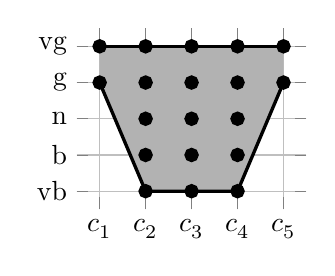
\begin{tikzpicture}
\begin{axis}[width = 4.5cm, ytick = {-2,-1,0,1,2}, xtick = {1,2,3,4,5}, xmin = 0.5, xmax = 5.500000, ymin = -2.5, ymax = 2.5, axis line style = {draw = none}, xmajorgrids, ymajorgrids, separate axis lines, yticklabels = {vb, b, n, g, vg}, xticklabels = {$c_1$,$c_2$,$c_3$,$c_4$,$c_5$}]
\addplot[name path = A, black, no markers, solid, very thick]
coordinates {
	(1,2)
	(2,2)
	(3,2)
	(4,2)
	(5,2)
};
\addplot[name path = B, black, no markers, solid, very thick]
coordinates {
	(1,1)
	(2,-2)
	(3,-2)
	(4,-2)
	(5,1)
};
\addplot[name path = C, black, mark = *, only marks, very thick]
coordinates {
	(1,1)
	(1,2)
	(2,-2)
	(2,-1)
	(2,0)
	(2,1)
	(2,2)
	(3,-2)
	(3,-1)
	(3,0)
	(3,1)
	(3,2)
	(4,-2)
	(4,-1)
	(4,0)
	(4,1)
	(4,2)
	(5,1)
	(5,2)
};
\addplot[white!70!black] fill between[of=A and B];
\end{axis}
\end{tikzpicture}

\noindent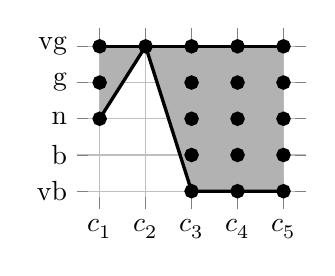
\begin{tikzpicture}
\begin{axis}[width = 4.5cm, ytick = {-2,-1,0,1,2}, xtick = {1,2,3,4,5}, xmin = 0.5, xmax = 5.500000, ymin = -2.5, ymax = 2.5, axis line style = {draw = none}, xmajorgrids, ymajorgrids, separate axis lines, yticklabels = {vb, b, n, g, vg}, xticklabels = {$c_1$,$c_2$,$c_3$,$c_4$,$c_5$}]
\addplot[name path = A, black, no markers, solid, very thick]
coordinates {
	(1,2)
	(2,2)
	(3,2)
	(4,2)
	(5,2)
};
\addplot[name path = B, black, no markers, solid, very thick]
coordinates {
	(1,0)
	(2,2)
	(3,-2)
	(4,-2)
	(5,-2)
};
\addplot[name path = C, black, mark = *, only marks, very thick]
coordinates {
	(1,0)
	(1,1)
	(1,2)
	(2,2)
	(3,-2)
	(3,-1)
	(3,0)
	(3,1)
	(3,2)
	(4,-2)
	(4,-1)
	(4,0)
	(4,1)
	(4,2)
	(5,-2)
	(5,-1)
	(5,0)
	(5,1)
	(5,2)
};
\addplot[white!70!black] fill between[of=A and B];
\end{axis}
\end{tikzpicture}
	
		\vspace{1ex}
		\hrule
		\vspace{1ex}
		
	{\bf Bad Contributors}
	
		\vspace{1ex}
		\hrule
		\vspace{1ex}
	
\noindent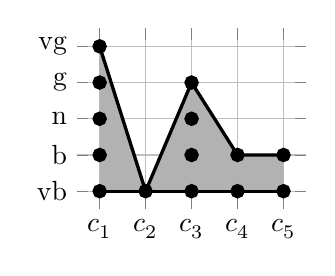
\begin{tikzpicture}
\begin{axis}[width = 4.5cm, ytick = {-2,-1,0,1,2}, xtick = {1,2,3,4,5}, xmin = 0.5, xmax = 5.500000, ymin = -2.5, ymax = 2.5, axis line style = {draw = none}, xmajorgrids, ymajorgrids, separate axis lines, yticklabels = {vb, b, n, g, vg}, xticklabels = {$c_1$,$c_2$,$c_3$,$c_4$,$c_5$}]
\addplot[name path = A, black, no markers, solid, very thick]
coordinates {
	(1,2)
	(2,-2)
	(3,1)
	(4,-1)
	(5,-1)
};
\addplot[name path = B, black, no markers, solid, very thick]
coordinates {
	(1,-2)
	(2,-2)
	(3,-2)
	(4,-2)
	(5,-2)
};
\addplot[name path = C, black, mark = *, only marks, very thick]
coordinates {
	(1,-2)
	(1,-1)
	(1,0)
	(1,1)
	(1,2)
	(2,-2)
	(3,-2)
	(3,-1)
	(3,0)
	(3,1)
	(4,-2)
	(4,-1)
	(5,-2)
	(5,-1)
};
\addplot[white!70!black] fill between[of=A and B];
\end{axis}
\end{tikzpicture}
\noindent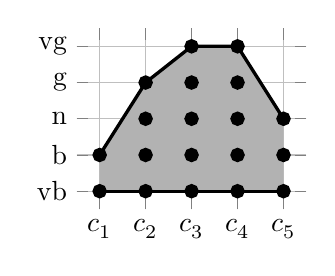
\begin{tikzpicture}
\begin{axis}[width = 4.5cm, ytick = {-2,-1,0,1,2}, xtick = {1,2,3,4,5}, xmin = 0.5, xmax = 5.500000, ymin = -2.5, ymax = 2.5, axis line style = {draw = none}, xmajorgrids, ymajorgrids, separate axis lines, yticklabels = {vb, b, n, g, vg}, xticklabels = {$c_1$,$c_2$,$c_3$,$c_4$,$c_5$}]
\addplot[name path = A, black, no markers, solid, very thick]
coordinates {
	(1,-1)
	(2,1)
	(3,2)
	(4,2)
	(5,0)
};
\addplot[name path = B, black, no markers, solid, very thick]
coordinates {
	(1,-2)
	(2,-2)
	(3,-2)
	(4,-2)
	(5,-2)
};
\addplot[name path = C, black, mark = *, only marks, very thick]
coordinates {
	(1,-2)
	(1,-1)
	(2,-2)
	(2,-1)
	(2,0)
	(2,1)
	(3,-2)
	(3,-1)
	(3,0)
	(3,1)
	(3,2)
	(4,-2)
	(4,-1)
	(4,0)
	(4,1)
	(4,2)
	(5,-2)
	(5,-1)
	(5,0)
};
\addplot[white!70!black] fill between[of=A and B];
\end{axis}
\end{tikzpicture}
\noindent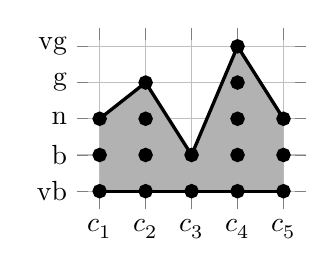
\begin{tikzpicture}
\begin{axis}[width = 4.5cm, ytick = {-2,-1,0,1,2}, xtick = {1,2,3,4,5}, xmin = 0.5, xmax = 5.500000, ymin = -2.5, ymax = 2.5, axis line style = {draw = none}, xmajorgrids, ymajorgrids, separate axis lines, yticklabels = {vb, b, n, g, vg}, xticklabels = {$c_1$,$c_2$,$c_3$,$c_4$,$c_5$}]
\addplot[name path = A, black, no markers, solid, very thick]
coordinates {
	(1,0)
	(2,1)
	(3,-1)
	(4,2)
	(5,0)
};
\addplot[name path = B, black, no markers, solid, very thick]
coordinates {
	(1,-2)
	(2,-2)
	(3,-2)
	(4,-2)
	(5,-2)
};
\addplot[name path = C, black, mark = *, only marks, very thick]
coordinates {
	(1,-2)
	(1,-1)
	(1,0)
	(2,-2)
	(2,-1)
	(2,0)
	(2,1)
	(3,-2)
	(3,-1)
	(4,-2)
	(4,-1)
	(4,0)
	(4,1)
	(4,2)
	(5,-2)
	(5,-1)
	(5,0)
};
\addplot[white!70!black] fill between[of=A and B];
\end{axis}
\end{tikzpicture}
	
		\vspace{1ex}
		\hrule
	
    \caption{Assignment rules for good and bad contributors from the perspective of \DB.}\label{fig:ex2-rules-reduced1}
\end{figure}

\DB felt that the model was slightly inaccurate, and decided to tweak the first two rules of the Good category by raising the boundary of the second criterion from $very\ bad$ to $bad$, as he felt that being neutrally committed to the project and having a clear inability to work with others would not be a characteristic of a good team member, regardless of all other factors. In the Bad category, \DB also felt that a very committed team member should not be in the Bad category, regardless of other poor evaluations, but qualified this by mentioning that if the commitment were to fall to neutral, this would indeed be a Bad team member. The second and third rules in the Bad category were adjusted accordingly by lowering slightly the good evaluation on the second criterion to a neutral one. The final model is illustrated in Figure~\ref{fig:ex2-model4}, while the assignment rules derived from it are presented in Figure~\ref{fig:ex2-rules-reduced2}.

\begin{figure}
\centering

\begin{minipage}[c]{0.4\columnwidth}
\vspace{0pt}
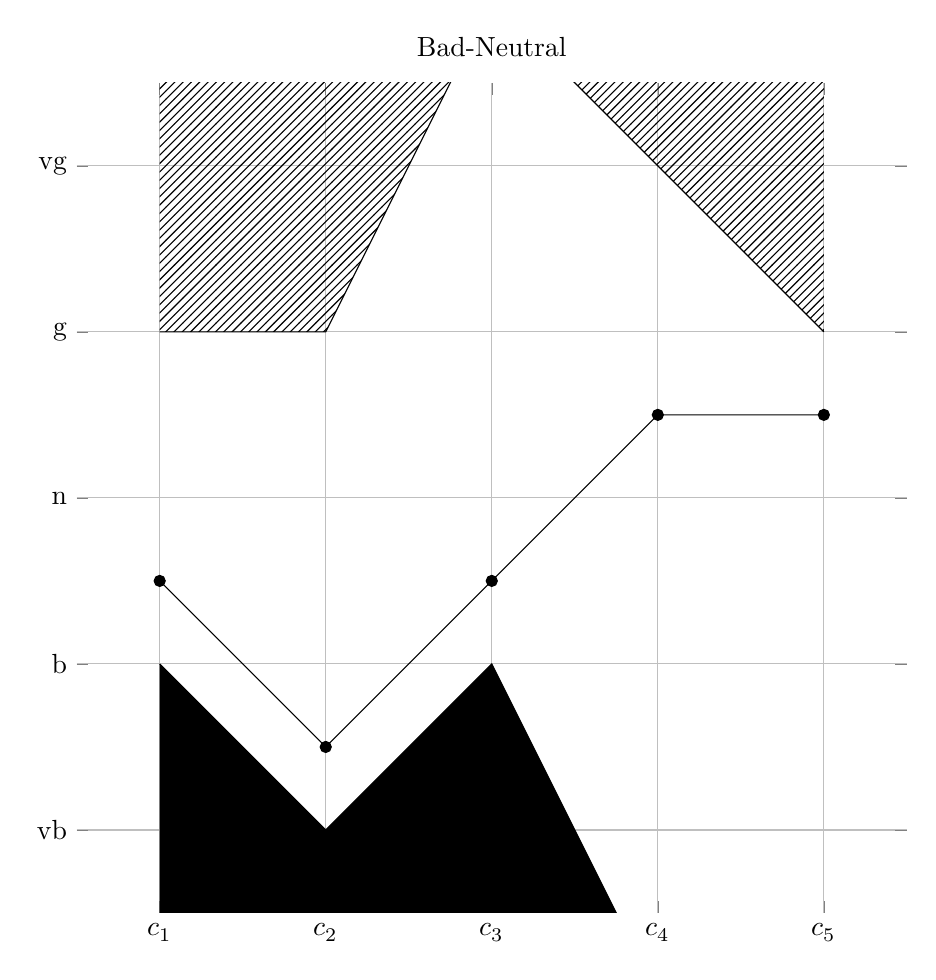
\begin{tikzpicture}
\begin{axis}[title ={Bad-Neutral}, height=\textwidth,width=\textwidth, xmin = 0.5, xmax = 5.5, ymin = -2.5, ymax = 2.5, every axis x label/.style={at={(ticklabel* cs:0.97)},anchor=south},xtick={1,2,3,4,5}, xticklabels={$c_1$,$c_2$,$c_3$,$c_4$,$c_5$}, ytick={-2,-1,0,1,2}, xmajorgrids = true, axis line style = { draw = none }, yticklabels = {vb, b, n, g, vg}, ymajorgrids = true]
\addplot[name path=T]
coordinates {
	(1,3)
	(2,3)
	(3,3)
	(4,3)
	(5,3)
};
\addplot[name path=B]
coordinates {
	(1,-3)
	(2,-3)
	(3,-3)
	(4,-3)
	(5,-3)
};
\addplot[name path=P, black, solid, mark = *]
coordinates {
	(1,-0.5)
	(2,-1.5)
	(3,-0.5)
	(4,0.5)
	(5,0.5)
};
\addplot[name path=V]
coordinates {
	(1,-1)
	(2,-2)
	(3,-1)
	(4,-3)
	(5,-3)
};
\addplot[name path=D]
coordinates {
	(1,1)
	(2,1)
	(3,3)
	(4,2)
	(5,1)
};
\addplot[black] fill between[of=V and B];
\addplot[pattern = north east lines] fill between[of=D and T];
\end{axis}
\end{tikzpicture}
\end{minipage}
\begin{minipage}[c]{0.4\columnwidth}
\vspace{0pt}

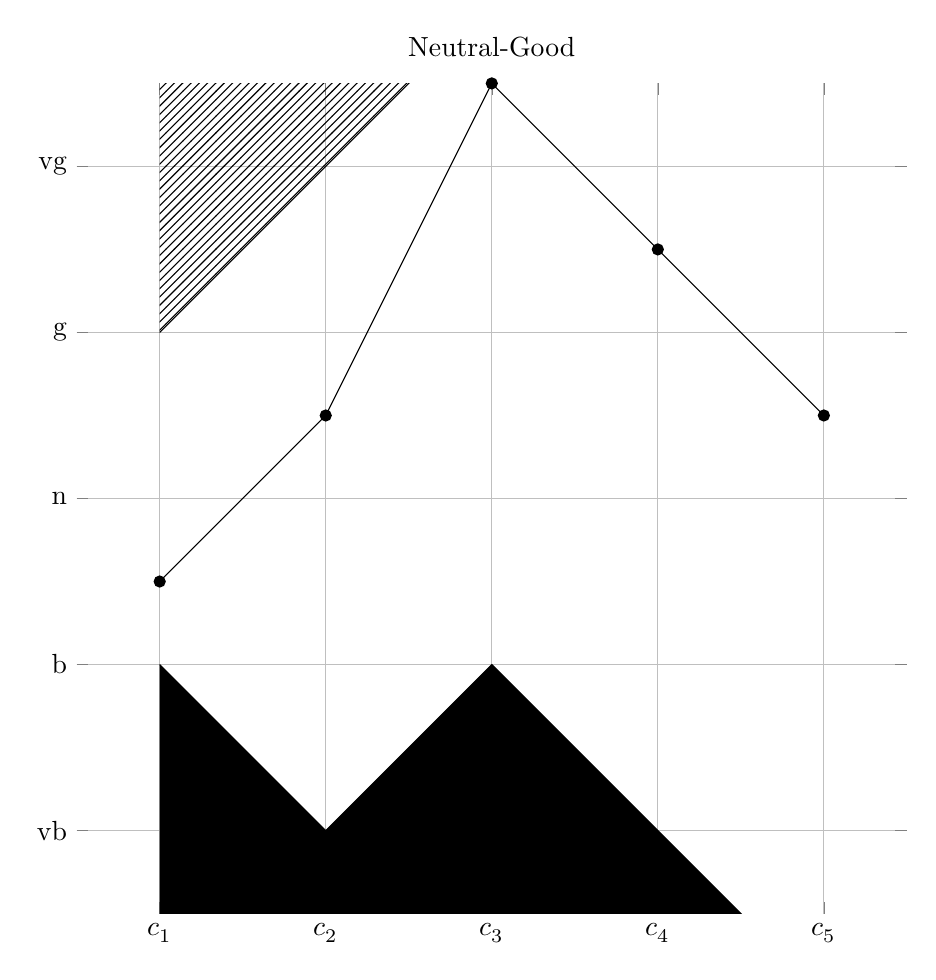
\begin{tikzpicture}
\begin{axis}[title ={Neutral-Good}, height=\textwidth,width=\textwidth, xmin = 0.5, xmax = 5.5, ymin = -2.5, ymax = 2.5, every axis x label/.style={at={(ticklabel* cs:0.97)},anchor=south},xtick={1,2,3,4,5}, xticklabels={$c_1$,$c_2$,$c_3$,$c_4$,$c_5$}, ytick={-2,-1,0,1,2}, xmajorgrids = true, axis line style = { draw = none }, yticklabels = {vb, b, n, g, vg}, ymajorgrids = true]
\addplot[name path=T]
coordinates {
	(1,3)
	(2,3)
	(3,3)
	(4,3)
	(5,3)
};
\addplot[name path=B]
coordinates {
	(1,-3)
	(2,-3)
	(3,-3)
	(4,-3)
	(5,-3)
};
\addplot[name path=P, black, solid, mark = *]
coordinates {
	(1,-0.5)
	(2,0.5)
	(3,2.5)
	(4,1.5)
	(5,0.5)
};
\addplot[name path=V]
coordinates {
	(1,-1)
	(2,-2)
	(3,-1)
	(4,-2)
	(5,-3)
};
\addplot[name path=D]
coordinates {
	(1,1)
	(2,2)
	(3,3)
	(4,3)
	(5,3)
};
\addplot[black] fill between[of=V and B];
\addplot[pattern = north east lines] fill between[of=D and T];
\end{axis}
\end{tikzpicture}
\end{minipage}
\begin{minipage}[c]{0.07\columnwidth}
\vspace{0pt}

\begin{tabular}{c|c}
$\lambda$ & 0.55 \\\hline
$c_1$ & 0.40 \\
$c_2$ & 0.15 \\
$c_3$ & 0.15 \\
$c_4$ & 0.15 \\
$c_5$ & 0.15
\end{tabular}
\end{minipage}

\caption{Final preference model of \DB (MR-Sort with vetoes weakened by dictators).}\label{fig:ex2-model4}
\end{figure}

\begin{figure}
	\centering
	
		\hrule
		\vspace{1ex}
	
	{\bf Good Contributors}
	
		\vspace{1ex}
		\hrule
		\vspace{1ex}

\noindent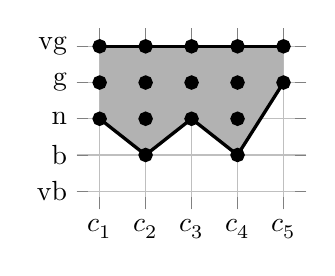
\begin{tikzpicture}
\begin{axis}[width = 4.5cm, ytick = {-2,-1,0,1,2}, xtick = {1,2,3,4,5}, xmin = 0.5, xmax = 5.500000, ymin = -2.5, ymax = 2.5, axis line style = {draw = none}, xmajorgrids, ymajorgrids, separate axis lines, yticklabels = {vb, b, n, g, vg}, xticklabels = {$c_1$,$c_2$,$c_3$,$c_4$,$c_5$}]
\addplot[name path = A, black, no markers, solid, very thick]
coordinates {
	(1,2)
	(2,2)
	(3,2)
	(4,2)
	(5,2)
};
\addplot[name path = B, black, no markers, solid, very thick]
coordinates {
	(1,0)
	(2,-1)
	(3,0)
	(4,-1)
	(5,1)
};
\addplot[name path = C, black, mark = *, only marks, very thick]
coordinates {
	(1,0)
	(1,1)
	(1,2)
	(2,-1)
	(2,0)
	(2,1)
	(2,2)
	(3,0)
	(3,1)
	(3,2)
	(4,-1)
	(4,0)
	(4,1)
	(4,2)
	(5,1)
	(5,2)
};
\addplot[white!70!black] fill between[of=A and B];
\end{axis}
\end{tikzpicture}
\noindent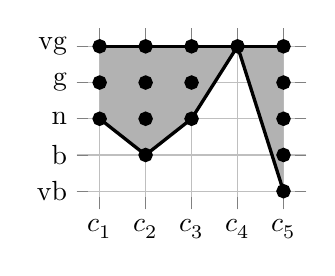
\begin{tikzpicture}
\begin{axis}[width = 4.5cm, ytick = {-2,-1,0,1,2}, xtick = {1,2,3,4,5}, xmin = 0.5, xmax = 5.500000, ymin = -2.5, ymax = 2.5, axis line style = {draw = none}, xmajorgrids, ymajorgrids, separate axis lines, yticklabels = {vb, b, n, g, vg}, xticklabels = {$c_1$,$c_2$,$c_3$,$c_4$,$c_5$}]
\addplot[name path = A, black, no markers, solid, very thick]
coordinates {
	(1,2)
	(2,2)
	(3,2)
	(4,2)
	(5,2)
};
\addplot[name path = B, black, no markers, solid, very thick]
coordinates {
	(1,0)
	(2,-1)
	(3,0)
	(4,2)
	(5,-2)
};
\addplot[name path = C, black, mark = *, only marks, very thick]
coordinates {
	(1,0)
	(1,1)
	(1,2)
	(2,-1)
	(2,0)
	(2,1)
	(2,2)
	(3,0)
	(3,1)
	(3,2)
	(4,2)
	(5,-2)
	(5,-1)
	(5,0)
	(5,1)
	(5,2)
};
\addplot[white!70!black] fill between[of=A and B];
\end{axis}
\end{tikzpicture}
\noindent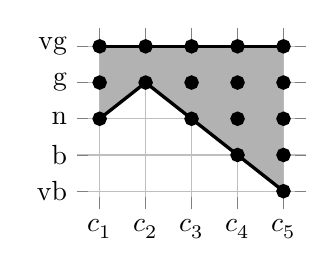
\begin{tikzpicture}
\begin{axis}[width = 4.5cm, ytick = {-2,-1,0,1,2}, xtick = {1,2,3,4,5}, xmin = 0.5, xmax = 5.500000, ymin = -2.5, ymax = 2.5, axis line style = {draw = none}, xmajorgrids, ymajorgrids, separate axis lines, yticklabels = {vb, b, n, g, vg}, xticklabels = {$c_1$,$c_2$,$c_3$,$c_4$,$c_5$}]
\addplot[name path = A, black, no markers, solid, very thick]
coordinates {
	(1,2)
	(2,2)
	(3,2)
	(4,2)
	(5,2)
};
\addplot[name path = B, black, no markers, solid, very thick]
coordinates {
	(1,0)
	(2,1)
	(3,0)
	(4,-1)
	(5,-2)
};
\addplot[name path = C, black, mark = *, only marks, very thick]
coordinates {
	(1,0)
	(1,1)
	(1,2)
	(2,1)
	(2,2)
	(3,0)
	(3,1)
	(3,2)
	(4,-1)
	(4,0)
	(4,1)
	(4,2)
	(5,-2)
	(5,-1)
	(5,0)
	(5,1)
	(5,2)
};
\addplot[white!70!black] fill between[of=A and B];
\end{axis}
\end{tikzpicture}
\noindent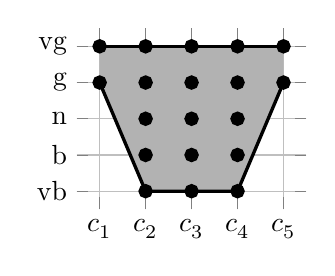
\begin{tikzpicture}
\begin{axis}[width = 4.5cm, ytick = {-2,-1,0,1,2}, xtick = {1,2,3,4,5}, xmin = 0.5, xmax = 5.500000, ymin = -2.5, ymax = 2.5, axis line style = {draw = none}, xmajorgrids, ymajorgrids, separate axis lines, yticklabels = {vb, b, n, g, vg}, xticklabels = {$c_1$,$c_2$,$c_3$,$c_4$,$c_5$}]
\addplot[name path = A, black, no markers, solid, very thick]
coordinates {
	(1,2)
	(2,2)
	(3,2)
	(4,2)
	(5,2)
};
\addplot[name path = B, black, no markers, solid, very thick]
coordinates {
	(1,1)
	(2,-2)
	(3,-2)
	(4,-2)
	(5,1)
};
\addplot[name path = C, black, mark = *, only marks, very thick]
coordinates {
	(1,1)
	(1,2)
	(2,-2)
	(2,-1)
	(2,0)
	(2,1)
	(2,2)
	(3,-2)
	(3,-1)
	(3,0)
	(3,1)
	(3,2)
	(4,-2)
	(4,-1)
	(4,0)
	(4,1)
	(4,2)
	(5,1)
	(5,2)
};
\addplot[white!70!black] fill between[of=A and B];
\end{axis}
\end{tikzpicture}

\noindent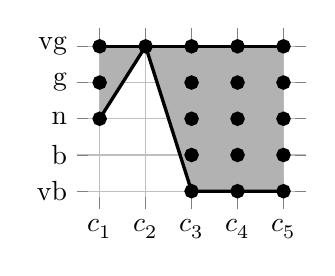
\begin{tikzpicture}
\begin{axis}[width = 4.5cm, ytick = {-2,-1,0,1,2}, xtick = {1,2,3,4,5}, xmin = 0.5, xmax = 5.500000, ymin = -2.5, ymax = 2.5, axis line style = {draw = none}, xmajorgrids, ymajorgrids, separate axis lines, yticklabels = {vb, b, n, g, vg}, xticklabels = {$c_1$,$c_2$,$c_3$,$c_4$,$c_5$}]
\addplot[name path = A, black, no markers, solid, very thick]
coordinates {
	(1,2)
	(2,2)
	(3,2)
	(4,2)
	(5,2)
};
\addplot[name path = B, black, no markers, solid, very thick]
coordinates {
	(1,0)
	(2,2)
	(3,-2)
	(4,-2)
	(5,-2)
};
\addplot[name path = C, black, mark = *, only marks, very thick]
coordinates {
	(1,0)
	(1,1)
	(1,2)
	(2,2)
	(3,-2)
	(3,-1)
	(3,0)
	(3,1)
	(3,2)
	(4,-2)
	(4,-1)
	(4,0)
	(4,1)
	(4,2)
	(5,-2)
	(5,-1)
	(5,0)
	(5,1)
	(5,2)
};
\addplot[white!70!black] fill between[of=A and B];
\end{axis}
\end{tikzpicture}
	
		\vspace{1ex}
		\hrule
		\vspace{1ex}
		
	{\bf Bad Contributors}
	
		\vspace{1ex}
		\hrule
		\vspace{1ex}

\noindent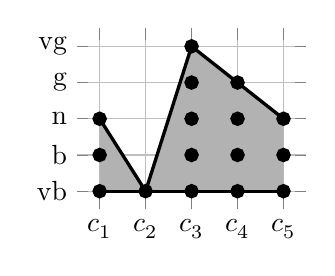
\begin{tikzpicture}
\begin{axis}[width = 4.5cm, ytick = {-2,-1,0,1,2}, xtick = {1,2,3,4,5}, xmin = 0.5, xmax = 5.500000, ymin = -2.5, ymax = 2.5, axis line style = {draw = none}, xmajorgrids, ymajorgrids, separate axis lines, yticklabels = {vb, b, n, g, vg}, xticklabels = {$c_1$,$c_2$,$c_3$,$c_4$,$c_5$}]
\addplot[name path = A, black, no markers, solid, very thick]
coordinates {
	(1,0)
	(2,-2)
	(3,2)
	(4,1)
	(5,0)
};
\addplot[name path = B, black, no markers, solid, very thick]
coordinates {
	(1,-2)
	(2,-2)
	(3,-2)
	(4,-2)
	(5,-2)
};
\addplot[name path = C, black, mark = *, only marks, very thick]
coordinates {
	(1,-2)
	(1,-1)
	(1,0)
	(2,-2)
	(3,-2)
	(3,-1)
	(3,0)
	(3,1)
	(3,2)
	(4,-2)
	(4,-1)
	(4,0)
	(4,1)
	(5,-2)
	(5,-1)
	(5,0)
};
\addplot[white!70!black] fill between[of=A and B];
\end{axis}
\end{tikzpicture}
\noindent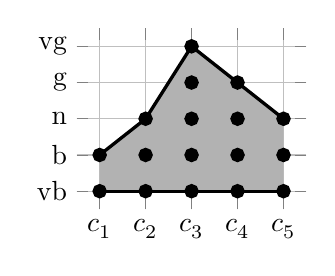
\begin{tikzpicture}
\begin{axis}[width = 4.5cm, ytick = {-2,-1,0,1,2}, xtick = {1,2,3,4,5}, xmin = 0.5, xmax = 5.500000, ymin = -2.5, ymax = 2.5, axis line style = {draw = none}, xmajorgrids, ymajorgrids, separate axis lines, yticklabels = {vb, b, n, g, vg}, xticklabels = {$c_1$,$c_2$,$c_3$,$c_4$,$c_5$}]
\addplot[name path = A, black, no markers, solid, very thick]
coordinates {
	(1,-1)
	(2,0)
	(3,2)
	(4,1)
	(5,0)
};
\addplot[name path = B, black, no markers, solid, very thick]
coordinates {
	(1,-2)
	(2,-2)
	(3,-2)
	(4,-2)
	(5,-2)
};
\addplot[name path = C, black, mark = *, only marks, very thick]
coordinates {
	(1,-2)
	(1,-1)
	(2,-2)
	(2,-1)
	(2,0)
	(3,-2)
	(3,-1)
	(3,0)
	(3,1)
	(3,2)
	(4,-2)
	(4,-1)
	(4,0)
	(4,1)
	(5,-2)
	(5,-1)
	(5,0)
};
\addplot[white!70!black] fill between[of=A and B];
\end{axis}
\end{tikzpicture}
\noindent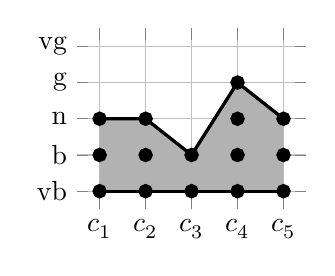
\begin{tikzpicture}
\begin{axis}[width = 4.5cm, ytick = {-2,-1,0,1,2}, xtick = {1,2,3,4,5}, xmin = 0.5, xmax = 5.500000, ymin = -2.5, ymax = 2.5, axis line style = {draw = none}, xmajorgrids, ymajorgrids, separate axis lines, yticklabels = {vb, b, n, g, vg}, xticklabels = {$c_1$,$c_2$,$c_3$,$c_4$,$c_5$}]
\addplot[name path = A, black, no markers, solid, very thick]
coordinates {
	(1,0)
	(2,0)
	(3,-1)
	(4,1)
	(5,0)
};
\addplot[name path = B, black, no markers, solid, very thick]
coordinates {
	(1,-2)
	(2,-2)
	(3,-2)
	(4,-2)
	(5,-2)
};
\addplot[name path = C, black, mark = *, only marks, very thick]
coordinates {
	(1,-2)
	(1,-1)
	(1,0)
	(2,-2)
	(2,-1)
	(2,0)
	(3,-2)
	(3,-1)
	(4,-2)
	(4,-1)
	(4,0)
	(4,1)
	(5,-2)
	(5,-1)
	(5,0)
};
\addplot[white!70!black] fill between[of=A and B];
\end{axis}
\end{tikzpicture}
	
		\vspace{1ex}
		\hrule
	
    \caption{Adjusted assignment rules for good and bad contributors from the perspective of \DB.}\label{fig:ex2-rules-reduced2}
\end{figure}

In the next section we will discuss the findings from these experiments, and what it implies about the methodology and its relevance to IS and management practitioners and scholars.


\section{Discussion}\label{sec:discussion}
\subsection{Evaluating team members\ldots and DMs}

In addition to the two DMs whose preferences were described in detail, %Section~\ref{sec:results:sub:model}
four other DMs participated. Table~\ref{tab:criteria} shows the criteria each selected as `important' or `very important' according to the second step of the methodology. % Section~\ref{sec:results:sub:subset}.

\begin{table}[h]
\centering
\caption{Important Criteria for DMs}\label{tab:criteria}
\begin{tabular}{c|c|c|c|c|c|c}
\multirow{2}{*}{Criteria} & \multicolumn{6}{c}{Decision makers}\\
& \GJ & \DB & \RH & \LD & \RQ & \XA\\\hline
Communication skills & & & \correct & & \correct & \correct \\
Commitment to the project &  \correct& \correct & \correct & \correct & \correct & \correct \\
Working with others & \correct & \correct & \correct & \correct & \correct & \correct \\
Pressure and stress related managing capacity & & & & \correct & \correct & \correct \\
Creativity & & & & & & \correct \\
Quantity of code produced & & & & \correct & & \\
Quality of code produced & \correct & \correct & \correct & & \correct & \correct \\
Global picture & \correct & \correct & \correct & \correct & \correct & \correct \\
Documentation and testing & \correct & \correct & \correct & \correct & \correct & \correct\\
Contributions on other aspects & & & \correct & \correct & & \\
\end{tabular}
\end{table}

Each of the dimensions were considered useful by at least one DM, while no DM considered all criteria necessary. We observe that the dimensions related to the commitment of contributors, their capacity to work together, their perspective of the project as a whole and their ability to document their work were unanimously considered important factors by all DMs. Furthermore, most were also concerned with the quality of code produced.

This result supports the premise of the article: if a set of variables can describe what is observable and important for evaluating a virtual team member, managers will only use a subset of these variables, and do not agree on what this subset is. Even when they agree on the subset of dimensions, the relative importance of the factors and the interactions between them will be adjudged differently, as shown in our experiment, illustrated with Figures~\ref{fig:ex1-rules-reduced} and \ref{fig:ex2-rules-reduced1}. While the protocol in both cases led to an MR-Sort with vetoes weakened by dictators, the resulting models and assignment rules were quite different.

\GJ placed a more or less equal emphasis on all five variables, requiring that a virtual team member be at least good on four out of five variables in order to fit in the Neutral or Good categories, veto and dictator effects notwithstanding. The ability to work with others was given slightly less weight than the other variables. For the first, third and fifth variables, the division revolved around a neutral evaluation, however only very bad performance on the remaining two variables was considered characteristic of a bad contributor. Several vetoes emerged, showing that a good contributor could not be very bad on any of the variables except the  global perspective on the project. However, even in this case, a very good global perspective could negate these very bad attributes. Finally, very bad code quality or documentation skills were enough to mark the contributor as Bad, provided a good global perspective was lacking.

%%% Added after MISQ submission
When we compare the model which emerged, shown in Figure~\ref{fig:ex1-model3}, to a model which might have been built based on his statements and his initial selection in the questionnaire, the MCDA technique has elicited a more detailed picture. Initially, \GJ put $c_1$, commitment to the project, as very important and other factors as important. but in the model we developed, which was validated by \GJ, $c_1$ is as important as $c_4$ and $c_5$, and slightly less important than $c_3$. This demonstrates that considering each factor in isolation can yield different results compared to when the DM is forced to take multiple important factors into consideration at once. As such, MCDA offers a solution to untangling priority when faced with multiple important criteria.
%%% end added after submission

\DB, on the other hand, had a very different perspective on contributor qualities, despite using the same five variables in his assessment. 
%%% Added after MISQ submission
Figure~\ref{fig:ex2-model4} shows \DB's final elicited model. 
%%% end added after submission
A large emphasis was placed on the first variable, commitment to the project, which could be paired with any of the remaining variables in order to form a majority coalition, leading to a contributor with performances at least as good as the category profile on these coalitions could be placed in either the Neutral or the Good category, ignoring for a moment the veto and dictator constructs. \DB's profiles on the first and last variables were identical to those of \GJ, but the levels of the remaining ones were different. In contrast to \GJ, \DB was less demanding on the second criterion and more critical on the third and fourth. With respect to the vetoes, \DB was less tolerant of bad performance on commitment and code quality, but readily tolerated very bad performance on the global perspective and documentation skills. Nevertheless, good performances on the first two and last variables served to negate any vetoes, whereas only good levels on project commitment and very good ones on working with others had the same effect of elevating profiles to Good.

%%% Added after MISQ submission
In his initial interview, \DB rated commitment to the project ($c_1$), ability to work with others ($c_2$), quality of code ($c_3$) and documentation and testing ($c_5$) and very important, and understanding of the tools, technologies, domain and process behind the project ($c_4$) as important. The eventual model showed that commitment to the project was in fact the single most important factor, contributing 40\% of the of the weight. The global picture was indeed a less important factor, but so was documentation. It is clear that a 5-item scale as in the questionnaire is insufficient to elicit the same level of detail, such as the extreme importance of $c_1$ relative to the other dimensions. The interview did provide additional information, as \DB stated emphatically that commitment to the project was the single most important factor, but from this alone we could not have inferred such a detailed model as the one which which eventually emerged.
%%% end added after submission

\subsection{Managerial and Theoretical implications}
\label{subsec:managerialimplic}

These results for our managerial preferences elicitation method regarding virtual team members leads to several implications. As initially stated, our goal was not to exhaustively identify all potential classes of managers based on their preferences, not even within the scope of FLOSS communities.

%%%% changes here %%%%
This work, however, provides several contributions to the IS literature and to the virtual team managers.

First it appears to indicate that even in the case of virtual teams, where a portion of the behaviors is unobservable, the DM can agree on the fact that a subset of elements, derived from the literature, is both observable and can be used to evaluate their team members. Of course this result is based on observations of only six DMs, and should be expanded through additional research.
Our work helps to go beyond the paradox raised by \cite{KayworthLeidner02} about both the non-statistical link between team manager characteristics and team performance, but also team leader importance in trust-building by exposing that there is no direct link, because managers are different and have different expectations.
%%%%%% end of modification

From a theoretical point of view, this may open a new area of research into the collection of data on a manager's expectations regarding team members in particular, and principal-agent modeling in general, especially from an IS point of view. Instead of trying to identify a good agent for the majority of managers through statistical inference, we propose to construct an individual preference model for every manager. As we have shown in our experiments, the managers may not agree on the same set of dimensions with which to evaluate their team members, and even when they do, the resulting preference models can be quite different.
We are confident that this approach would result in solid and actionable results regarding efficient teaming questions.

Regarding the application of the method to the IS field, the importance of trust-building and the role of the manager in doing so \citep{KayworthLeidner02}, through integrity and benevolence \citep{JarvenpaaKnollLeidner98}, has been identified. Therefore the first contact between the manager and the team, and the manager's communication of expectations are of utmost importance. This is where our work may provide solutions to practitioners. We have proposed a method and showed that this allows managers to better define what their evaluation criteria are. This model does not identify a single acceptable profile, but allows for team members to have different strengths and weaknesses, yet understand the relative importance of different attributes. Because the results are presented in a structured way, ambiguity is reduced and transparency is increased. This method can help not only in the team building phase, but also in subsequent coaching and in explaining the team manager's expectations.

To be fully useful, however, the implementation of our methodology requires improvement, both in terms of information system design and implementation and in terms of algorithmic efficiency in the construction of the models. In particular, we relied on repeated interviews with the DMs, and in a large-scale application of the method, interviews may only be warranted in the first iteration, when the manager's understanding of the process may be unclear. Automating the third step for subsequent iterations would greatly reduce the burden on the manager.

\subsection{Methodological implications and evolutions}\label{subsec:Methodofindings}

While the proposed methodology and its application to the context of integrating managerial preferences when evaluating team members served to show the possibilities of modeling the perspective of each DM, there are nevertheless several limitations which can be addressed in future work.

To begin with, we only explored the family of models based on outranking relations, MR-Sort and its extensions, although other families of models could be considered. The motivation behind the use of these models was based on the ordinal scales used to evaluate team members on the different criteria, and the fact that the DM often describes a good team member based on the member's outstanding characteristics rather than the average of all attributes. We have also assumed that the DM has accurate knowledge of the performance of each team member in all dimensions, although quantitative measures linked to each dimensions could be additionally considered, allowing the DM to judge unknown team members, for instance, in the context of a recruitment procedure.

Another limitation relates to the use of exact inference algorithms, which can only be used when the number of assignment examples is small. This prevented us from constructing the preference models of each manager in a single session and instead spread our interactions across a period of multiple weeks. Because of this, we also had to deal with the effects of bounded rationality, where the DM's judgments could become slightly inconsistent, changing perspective on the problem from one session to the next. In order to overcome this by accelerating the whole process, approximative inference methods could be explored.



\section{Conclusion}\label{sec:conclusion}
ost of the analyses we discussed used dump data because they are
rather complete on the contributors the most involved, especially
on the process part. But, as \citet{PreeceShneiderman09} claimed,
if more studied are still needed to understand the Reader-to-leader
process, these analyses may be completed with more qualitative studies
and surveys. We found very few works, and this one does not help for
that, on the non-text production collaboration, such as the one by
\citet{Viegas07} on the images producers. However, it is worth noting
that the results founds on the reasons to participate, the structure
of interaction and of governance seem close to the vision administrators
have from the inside of the Encyclopedia, \citep[See][on the interview of Swedish Wikipedia Administrators]{Mattus09}.

These results are also coherent with \citet{OstromHess06}'s framework
and description of the knowledge commons: if finding the community
is easier than other communities of practice (see, for instance, \citealp{MerriamCourtenayBaumgartner03}
on the access to a community of practice of which), there is a period
of apprenticeship, to do so, people are nested in small groups, dedicated
to topics they were concerned about since the beginning of their participation.
Some rules structure this community, but are constantly under discussion
and constantly evolving to adapt the project to its environment and
its participants.

As announced at the beginning of this article, we did not look at
the feedback loop of \citeauthor{HessOstrom06b}'s model, the impact
of Wikipedia on its environment. There are a very actual and active
discussions in the librarian and the teaching communities on how integrating
the encyclopedia in their professional practices. If we only tangented
these debates in this work, especially when looking at Wikipedia quality,
we hope that this article may help the discussants to better understand
how the project works. The discussion by \citet{Konieczny09b} of
Wikipedia being or not a ''social movement'' participates to the
same questioning about the impact of this collective action on the
society, on the way the knowledge is produced and transmitted, but
also to a broader discussion of the links between the contribution
to online open communities and the involvement of a job (on that respect,
see the discussion proposed by \citet{Brown08}, relying on \citet{Himanen02},
on open-source and Wikipedia participants, where he argued that these
hackers are creating new borders between work and leisure).

% What is Wikipedia, impact on society

Finally, being such a successful collective action of creation of
a common, Wikipedia has been taken as an emblem of the wisdom of the
crowd \citep{Surowiecki04}. It is a system, even if an imperfect
one, which allows more to produce and discuss knowledge, thus, in
that sense, empowering more than traditional encyclopedias \citep{HansenBerenteLyytinen09}.
This does not mean either that everybody has access to the process,
as the technological boundaries, but also the organizational ones
remain important, a pointed out by \citet{Hartelius10} and \citet{Pfister11}
as by \citet{Perovic09}. Does that mean, as these two authors debate,
that Wikipedia is a thinking machine which overcomes the human fallibility
thanks to a technical system, and thus institutes a socio-technical
expertise instead of the traditional scientific expertise, and a as
argued by \citet{Perovic09}, a world ''of contingency without irony,
knowledge without self-observation and learning without thinking,
a world enshrined by Wikipedia today.''? Does this ''flawed knowledge
communities'' \citep{RobertsPeters11}, which is always discussing
its perimeter, as \citet{Kostakis10} showed in his analysis of inclusionists
and delationists, or \citet{deLaat12} on his analysis of the rules
regulating new edition, the future deposit of the human knowledge?

In addition to the doubtful argument that a system of production may
replace another, comparing Wikipedia with traditional encyclopedias
may simply miss the point. As explained by \citet{Mattus09}: it has
to be seen as one entry, always evolving to access to knowledge, but
which may be combined with others (scientific references, traditional
encyclopedias), and used as a tool amongst others, and not, as was
the Encyclopédie, the deposit of the human knowledge. What Wikipedia
shows is the extension of the knowledge and of the sources of knowledge,
since the seventeenth century, and thus the never ending need to educate
the users to have a critical, scientific reading of any source of
knowledge.



% Acknowledgments here
\section*{ACKNOWLEDGMENT}%
% This work was supported, in part, by Science Foundation Ireland grants 10/CE/I1855 and 13/RC/2094  to Lero - the Irish Software Research Centre (\url{www.lero.ie}).

% We would like to thank the six FLOSS community managers who participated in this research and Pr. Mathieu Simonnet, who provided input on the modeling of psychological traits. We would also like to thank Dr. Brian Fitzgerald, Dr. Brian Butler, and our anonymous reviewers, who provided valuable feedback which made the paper stronger.


% Enter the text of acknowledgments here
% Leave this (end of acknowledgment)


% Appendix here
% Options are (1) APPENDIX (with or without general title) or 
%             (2) APPENDICES (if it has more than one unrelated sections)
% Outcomment the appropriate case if necessary
%
\section*{APPENDIX}\label{sec:appendix}
\renewcommand{\thesubsection}{\Alph{subsection}} %% Appendices get letters
\subsection{Mathematical Description of MR-Sort}\label{app:mrsort}

Let $A$ denote the finite set of decision alternatives (or members) and $J$ be a finite set of criteria indexes. The output 
evaluation scale contains $k$ qualitative levels, which means that the  alternatives are to be sorted into $k$ categories ($c_1$, \ldots, $c_k$), ordered by their desirability, from $c_1$ being the worst category to $c_k$ being the best one. Each category $c_h$ is defined by the performance of its lower frontier, or category limit, $b_{h-1}$ and its upper 
frontier $b_h$ of $B = \{b_0, \ldots b_{k}\}$. Each alternative $a\in A$, or category limit $b_h\in B$ is evaluated on any criterion through a function $g_j$, where $g_j(a)$ ($j\in J$) denotes the performance of the alternative $a$ on criterion $g_j$. 

%The performances of the $b_0$ category limit will be fixed to the worst possible evaluations on all criteria, so that any alternative may be assigned at least to category $c_1$, while the performances of the $b_k$ category limit will be fixed so that they are better than the best possible evaluations on all criteria, hence any alternative will be assigned at most to category $c_k$. We assume, without loss of generality, that the performances are supposed to be such that a higher value denotes a better performance. Furthermore, the performances on the frontiers are non-decreasing, i.e. $\forall j \in J, h \in 1..k: g_j(b_{h-1}) \leqslant g_j(b_h)$.

An alternative $a$ is assigned to the highest possible category $c_h$ such that $a$ outranks the category's lower frontier $b_{h-1}$. In the MR-Sort model, an alternative $a$ is said to outrank a frontier $b_{h-1}$ if and only if there is a sufficient coalition of criteria supporting the assertion ``$a$ is at least as good as $b_{h-1}$''. More precisely, 
binary relations $C_j$ are first defined to assess whether each criterion $g_j$ supports this statement:
\begin{equation}
	\forall j \in J, a \in A, h\in 1..k+1: C_j(a, b_{h-1}) =
\left\{\begin{array}{l}
 1 \mbox{, if } g_j(a) \geqslant g_j(b_{h-1}),\\
 0 \mbox{, otherwise.}
\end{array}\right.
\end{equation}
The coalition of criteria in favor of the outranking, $\forall a \in A, h\in 1..k+1$, which we denote with $C(a, b_{h-1})$, is then defined as:
\begin{equation}
	C(a, b_{h-1}) = \sum_{j \in J} w_j C_j(a, b_{h-1}),
\end{equation}
where $w_j$ is the weight of the criterion $g_j$. 
%, and $C_j(a, b_{h-1}) \in \{0, 1\}$ measures if $a$ is at least as good as $b_{h-1}$ from the point of view of the criterion $j$ or not: $C_j(a, b_{h-1}) = 1 \Leftrightarrow g_j(a) \geq g_j(b_{h-1})$, 0 otherwise. 
The weights are defined so that they are positive ($w_j \geqslant 0, \forall j\in J$) and sum up to one ($\sum_{j \in J} w_j = 1$). The coalition of criteria is compared to a majority threshold $l \in [0.5,1]$ extracted from the DM's preferences along with the weights. If $C(a, b_{h-1})<l$, the coalition is not sufficient and the alternative does not outrank the frontier $b_{h-1}$ and will therefore be assigned in a category below $c_h$.

\subsection{Initial Interview with DMs}\label{app:interview}

\begin{tabular}{p{3cm}p{12cm}}
Interviewer: 	&	Thank you for talking to me. This call is being recorded. Is that all right with you?\\
Interviewer:	&	I wanted to talk to you specifically about the [name] community, of which you are a community manager.\\
Interviewer:	&	The purpose this research is to try to identify the technical and behavioral attributes of a good contributor. Could you start by telling me some aspects or attributes of what makes for a good code contributor in this community?\\
Interviewer:	&	Can you state any of the attributes or characteristics that you consider to be bad in a contributor, that you would specifically not like to see?\\
Interviewer:	&	I am now giving you a list of potential attributes of contributors. Could you please indicate how important you find these attributes, and talk me through your thoughts as you do so?
[Provide questionnaire]\\

Interviewer:	&	Thank you. The follow-up question is: after reading this list, do you have any additional thoughts on what makes a good contributor or a bad contributor?\\
Interviewer:	&	Thank you for your time.\\
\end{tabular}



%
%   or 
%
%\begin{APPENDICES}
%\end{APPENDICES}

%\bigskip

% Endnotes here
\theendnotes

%\bigskip

% References here (outcomment the appropriate case) 

% CASE 1: BiBTeX used to constantly update the references 
%   (while the paper is being written).
\bibliographystyle{misq} % outcomment this and next line in Case 1
\bibliography{floss.bib,software.bib,volunteering.bib,research_methods.bib,thispaper.bib}

% CASE 2: BiBTeX used to generate mypaper.bbl (to be further fine tuned)
%\input{mypaper.bbl} % outcomment this line in Case 2
%% NB 2017.06.09: the following references require manual modifications due to a lack of editor, resulting in a double comma before the publisher name:
%% Beecham (2014 & 2015)
%% Carillo
%% Deshpande
%% Keertipata
%% Noll
%% Poo-Caamano
%% Roman-Gonzalez
%% Tsay
%% Zhou

\end{document}

